%SAVEDAT= 1453457093
\documentclass[11pt, a4paper]{article} 
\usepackage{slashed,jheppub,multirow,relsize,soul}
\usepackage[normalem]{ulem}
\usepackage{color}
\usepackage{subcaption}

\newcommand{\refeq}[1]{Eq.~(\ref{#1})}
\newcommand{\refeqs}[2]{Eqs.~(\ref{#1})~and~(\ref{#2})}
\newcommand{\refeqss}[3]{Eqs.~(\ref{#1}), (\ref{#2})~and~(\ref{#3})}
\newcommand{\reffig}[1]{Fig.~\ref{#1}}
\newcommand{\reffigs}[2]{Figs.~\ref{#1}~and~\ref{#2}}
\newcommand{\refsec}[1]{Section~\ref{#1}}
\newcommand{\refapp}[1]{Appendix~\ref{#1}}
\newcommand{\reftab}[1]{Table~\ref{#1}}
\newcommand{\refref}[1]{Ref.~\cite{#1}}
\newcommand{\refrefs}[2]{Refs.~\cite{#1}~and~\cite{#2}}

\def\abelian{abelian}
\def\nonabelian{non-abelian}
\def\lagrangian{lagrangian}
\def\eg{\emph{e.g.}}
\def\ie{\emph{i.e.}}
\def\aka{\emph{a.k.a.}}
\def\muboone{MicroBooNE}
\def\minerva{MINER$\nu$A}

%%%%%%% A few editorial macros. %%%%%%%

\newcommand{\lorem}{ \textcolor[rgb]{0.8,0.8,0.8}{Lorem ipsum dolor sit amet, constetur
adipiscing elit, sed do eiusmod tempor incididunt ut labore et dolore magna
aliqua. Ut enim ad minim veniam, quis nostrud exercitation ullamco laboris nisi
ut aliquip ex ea commodo consequat. Duis aute irure dolor in reprehenderit in
voluptate velit esse cillum dolore eu fugiat nulla pariatur. Excepteur sint
occaecat cupidatat non proident, sunt in culpa qui officia deserunt mollit anim
id est laborum.}}

\newcounter{CommentCount}
\setcounter{CommentCount}{1}

\newcommand{\marcom}[2]{\textsuperscript{\textcolor{#1}{\theCommentCount}}\marginpar{\textsuperscript{\textcolor{#1}{\theCommentCount}}\textcolor{#1}{{\small#1: #2}}}\stepcounter{CommentCount}}

\newcommand{\newtext}[2]{\textcolor{#1}{\ul{#2}}}

% Add your own colour down here... 
\definecolor{PB}{rgb}{0.9,0,0}
\definecolor{MARK}{rgb}{0.612, 0.153, 0.69}

%%%%%%%%%%%%%%%%%%%%%%%%%%%%%%%%%%%%%%%


\title{MeV sterile neutrino decay at the Fermilab Short-Baseline Neutrino complex}

\author{Peter Ballett,}
\author{Silvia Pascoli}
\author{and Mark Ross-Lonergan}

\affiliation{Institute for Particle Physics Phenomenology, Department of
Physics, Durham University, South Road, Durham DH1 3LE, United Kingdom}

\emailAdd{peter.ballett@durham.ac.uk}
\emailAdd{silvia.pascoli@durham.ac.uk}
\emailAdd{mark.ross-lonergan@durham.ac.uk}

\abstract{
%
We study the sensitivity of the Short-Baseline Neutrino (SBN) programme at
Fermilab to sterile neutrino decay in both a minimal extension and more generic
beyond the Standard Model scenarios. We provide estimates for the bounds that
the SBN can be expected to place on the parameter spaces of these models,
finding that the facility can in many cases extend existing bounds whilst, due
to the strong particle identification capabilities of liquid-Argon technology,
also place bounds on as yet unconstrained channels. We also highlight the
phenomenological potential of the particular design of the facility,
investigating how the interplay between the three detectors located at distinct
distances from the source can be used to distinguish between backgrounds and
signals in competing models.}

\begin{document} 

\maketitle

\section{Introduction}

The neutrino sector of the Standard Model (SM) is known to be incomplete. The
observation of oscillatory behaviour between neutrino flavour states suggests a
set of mass terms with relevant (flavour) off-diagonal terms. There are many
ways that have been suggested in the literature to explain neutrino masses from
a theoretical perspective, ranging from the popular see-saw scenarios to
radiative mass generation or even more involved constructions. It is ultimately
the role of phenomenology to find ways to distinguish between candidate models,
and see what can be learnt from the neutrino sector about the structure of BSM
physics.
%
Not all models, however, lend themselves to experimental searches. For example,
the canonical Type-I see-saw \cite{Minkowski:1977sc, GellMann:1980vs,
Mohapatra:1979ia} suggests the existence of new particles with masses around
$10^{12}$--$10^{15}$ GeV, well out of reach of modern experimental techniques. One
observable feature of some models is the presence of novel fermionic singlets
of the SM gauge group, which we shall refer to as sterile neutrinos. These will
generically mix with the `active' neutrinos of the SM and could alter neutrino
phenomenology at observable scales. 
%
A well known example of such an effect is the short-baseline disappearance
signature associated with a sterile neutrino with a mass around the eV scale. Such a state
would produce oscillatory effects over short distances and has been invoked to
solve the anomalies found at some short-baseline oscillation experiments.
Explaining all anomalies in an economical fashion appears challenging in these
models, but more data would be needed before a decision can be made as to their
role in the neutrino sector.

In this article, we study a complementary paradigm to the oscillatory sterile
neutrino models where sterile neutrinos exist, are produced in neutrino beams,
but have masses sufficiently large to prevent oscillatory effects with the
active neutrinos through loss of coherence (see \eg\ \refref{Akhmedov:2009rb}).
Due to the presence of mixing effects, these particles are not generically
expected to be stable and their subsequent decays have been enumerated
\cite{Atre:2009rg} and searched for in many previous experiments.
%
Our focus will be on the role of the Fermilab SBN programme \cite{Antonello:2015lea}
for the search for sterile neutrinos of this type.
%
This experimental facility comprises of three separate detectors placed in the
Booster Neutrino Beam (BNB) at different (short) baseline distances: SBND
(previously known as LAr1-ND) at 110~m from the target, \muboone\ at 470~m and
Icarus-T600 at 600~m.  All three detectors are filled with Liquid Argon (LAr)
giving unprecedented reconstruction and particle identification capabilities
allowing for significantly lower backgrounds than predecessor technologies. 
%
%\newtext{PB}{In addition to events arising from the BNB, the detectors of the
%SBN complex will also collect events associated with the NuMI beam, currently
%being used in the NO$\nu$A, MINER$\nu$A and MINOS+ experiments. This beam is
%off-axis with respect to the SBN detectors leading to significant kinematic
%differences.}
%
The SBN facility has a number of interesting features relevant to the search
for sterile neutrino decay:

\begin{enumerate}

\item The reconstruction and particle ID capabilities of LAr technology means
the SBN program provides an ideal scenario to study the decay in flight of
sterile neutrinos, a job which has traditionally been left for low-mass
detectors with corresponding low beam-related backgrounds. 
%
We will discuss how a very high level of background suppression can be obtained
through a simple cut-based analysis motivated by the kinematic properties
of a beam-based decay-in-flight signal. 

\item The presence of three detectors with distinct baselines allows for 
contrasting behaviour between different models of any excess events. Beam 
independent backgrounds, beam-based backgrounds, signals from oscillatory 
steriles and sterile neutrino decay all have different scaling behaviours 
with detector baseline distance and total mass. Making three measurements using 
the same technology but with varying baselines and masses allows for a clear 
contrast between the explanations of any excess of events.

\item The three detectors also allow for timing-based effects between 
the three detectors if the excess comes from a sterile neutrino decay 
model. As we will discuss in \refsec{sec:timing}, this means that a decaying 
sterile neutrino would have a very distinctive pattern of excess events at
SBN, unobservable to a facility with a single detector.

\item The excellent particle identification will allow for the investigation of
channels for which there are no published searches, only infered bounds based
on minimal theoretical models. We will discuss extended models of sterile decay
where the minimal model correlations between decay channels do not hold. This
means that there are no published bounds on some channels, and a decay rate in
a traditionally excluded region could be observed at the SBN complex. In the
absence of signal, the facility could of course place the first bounds on these
signatures of new physics.

\end{enumerate} 

\begin{table}[t!]
\centering
\begin{tabular}{| l || l | l | l | l |}
	\hline
	& PS-191 & SBND & $\mu$BooNE & ICARUS \\ \hline \hline
	POT	& $0.86 \times 10^{19}$	& $6.6 \times 10^{20}$	&	$13.2 \times 10^{20}$     &  $6.6 \times 10^{20}$ \\ \hline
	Volume	& $216\text{m}^3$	&	$80\text{m}^3$	&	$62\text{m}^3$	     &   $340\text{m}^3$	\\ \hline
	$\text{Baseline}^{-2}$	& $(128 	\text{m} )^{-2}$	&$(110 \text{m} )^{-2}$	&	$(470 \text{m} )^{-2}$			     & $(600 \text{m} )^{-2}$	  \\ \hline
Ratio/PS-191 & - 	& 38.5 	& 3.3	& 5.5\\ \hline
\end{tabular}

\caption{\label{tab:exposure} A comparison of the exposure at each SBN detector compared to 
the PS-191 experiment. All detectors see larger numbers of events than PS-191, while SBND 
sees the largest enhancement of a factor of $38.5$; this is predominately due to proximity of the detector to source.}

\end{table}

Decaying heavy sterile neutrinos have been searched for at many experiments
since the early 1970s \cite{}. In the mass range of interest for SBN, the
strongest bounds on sterile which mix with electron and muon neutrinos come
from PS-191 \cite{Bernardi:1985ny}, which ran at CERN from 1983 to 1985. 
% 
We can estimate the sensitivity of the three SBN detectors and how they will
compare to PS-191 by a simple exposure calculation. PS-191 was located 128m
downstream of the target and $2.3^\circ$ (40 mrads) off axis, obtained $0.86
\times 10^{19}$ POT over the course of its run-time, and had a total detector
volume of $6\times3\times12 = 216 \text{m}^3$. The total number of events
scales as POT $\times$ Vol $\times$ $R^{-2}$ and we compare the three
facilities to PS-191 in \reftab{tab:exposure}. We see that all facilties expect
a larger exposure, with SBND seeing the largest enhancement by a factor of
around $40$.
%
In addition to the larger exposure, there is also an enhancement of the
expected decay events at SBN due to its lower beam energy. The steriles at SBN
are produced by the 8 GeV BNB beam and have a softer spectrum than those
produced by the 19.2 GeV proton synchrotron beam used at PS-191. This leads to
an increased number of expected decay events as the probability of the sterile
to subsequently decay scales as $1/E_\nu$. Thus we expect that the SBN
facilities to see more events than PS-191 even if their exposures were
identical. 
%
However, as mentioned above, PS-191 was purposefully built to search for deacys
in flight of heavy fermions and in order to minimize the background induced by
active neutrino scattering, the total mass of the detector was chosen to be
small (approximately $20$ ton). The SBN detectors, on the other hand, have been
designed to study neutrino scattering, which is reflected in their larger
masses ($112$, $66.6$ and $476$ tons respectively). Therefore, from these
general scale arguments, we expect SBN to see a greater number of decay events
than PS-191 but to also see a greater background. 
%
To understand the sensitivity of SBN to heavy sterile decay, we must therefore
show that background rejection capability of LAr is sufficiently well
understood. This will be the focus on \refsec{sec:bg}.

\section{Sterile neutrino decay}

A gauge-singlet fermion will generally be unobservable by all non-gravitational
means unless it mixes with the active neutrino sector. The presence of mixing
introduces a range of possible observable signatures depending on the magnitude
of the sterile mass and its mixing to the active sector. 

The most general renormalizable \lagrangian\ extending the SM to include a
single novel gauge-singlet fermion $N$ is given by
%
\begin{align}   \mathcal{L} = \mathcal{L}_\text{SM} +
\overline{N}i\slashed{\partial}N+ \frac{\mu}{2} \overline{N^\text{c}}N  +
y_\alpha\overline{L}_\alpha\tilde{H} N + y_\alpha^*
\overline{N}\widetilde{H}^*L_\alpha,\label{eq:minimallag} \end{align}
%
where $y_\alpha$ denote Yukawa couplings and $\mu$ a Majorana mass term for
$N$. The extension to multiple new fermions involves promoting $y$ and $\mu$ to
matrices with indices for the new states, but will offer no real
phenomenological difference in the current work.\footnote{The minimal single
$N$ extension does not allow for the observed masses of the neutrinos, as the
mass matrix is rank 1. We assume that an appropriate extension has been
introduced to satisfy neutrino oscillation data while introducing no new
dynamics at the energy scales of interest.} Much work has been done
understanding the phenomenology of novel neutral states, which varies
significantly over their large parameter spaces. 
%
If these particles have masses around $10^{15}$ GeV they could provide a
natural way to suppress the size of active neutrino masses through the Type I
or III see-saw mechanisms \cite{Minkowski:1977sc, GellMann:1980vs,
Mohapatra:1979ia}. A lighter neutral fermion, with a mass around the keV scale,
remains a promising dark matter candidate \cite{Adhikari:2016bei}. A synthesis
of these ideas is found in the so-called $\nu$MSM which simultanesouly can
explain dark matter, neutrino massesand successful baryogenesis
\cite{Asaka:2005pn}. 
%
If the sterile gets lighter still, with masses at the eV scale or below, an
important observable effects might exist in neutrino oscillation experiments.
Indeed, eV scale particles have been proposed to alleviate short-baseline
oscillation anomalies; although, no minimal solution seems to provide a
compelling universal improvement to the current data \cite{Kopp:2013vaa}. 
%

For steriles which are light enough to be produced in a neutrino beam,
typically with masses below the $D$-meson mass scale $m_\text{s} \lesssim
2$~GeV, there is a qualitative divide in their phenomenology somewhere between
keV and eV energies. If the sterile neutrinos are massive enough for their
mass-splittings between the light neutrinos to be larger than the wavepacket
uncertainty associated with the production mechanism, they no longer oscillate
\cite{Akhmedov:2009rb}.  
%
Once oscillation is suppressed, neutral particles produced in the beam will
propagate towards the detector and may be observed by their subsequent decay
into SM particles. Experiments seeking to measure such decays have been
performed for many years, and are generally known as beam dump experiments
where proton collisions with a target produce particles to be observed
down-wind of the source \cite{CooperSarkar:1985nh, Bergsma:1985is,
Vaitaitis:1999wq, Bernardi:1985ny, Bernardi:1987ek, Anelli:2015pba,
Alekhin:2015byh}. It has been pointed out that the difference between a beam
dump and a conventional neutrino beam is more a matter of philosophy, and we
can expect many experiments to have some sensitivity to novel heavy states
\cite{Gorbunov:2007ak, Asaka:2012bb, Adams:2013qkq}. 
%
For the BNB, we can estimate the mass at which this decoupling occurs as
follows: the decay pipe for BNB is around $50$~m in length, which is
considerably shorter than the decay lengths of the mesons in the beam.
Therefore this length defines the wavepacket width at production.  The relevant
parameter is the decoherence parameter \cite{Akhmedov:2009rb, Hernandez:2011rs}
%
\[  \xi = 2\pi \frac{\lambda_\text{d}}{\lambda_\nu}, \]
%
where $\lambda_\text{d} = 50$~m and $\lambda_\nu$ is the standard neutrino
oscillation length $\lambda_\nu = \Delta m^2/4E_\nu$. For $\xi\gg1$ the wave
packet is insufficiently broad to accomodate a coherence superposition of the
heavy and light neutrino states. We estimate that this occurs at 
%
\[  \Delta m^2 \gtrsim 20~\text{eV}^2. \] 
%
In this article we study the region of MeV scale sterile masses. These are
heavy enough to forbid oscillatory effects while light enough to be have
significant production from the meson decays associated with a conventional
neutrino beam. 

The observable signature in this model is the direct decay of the new fermion
into SM particles. In the minimal \lagrangian\ in \refeq{eq:minimallag}, the
only direct couplings to new sterile fermions are neutrino Higgs interactions.
However, these couplings generate off-diagonal neutrino bilinears below the
electroweak symmetry breaking scale, which leads to mass mixing between the
$4+$ flavours of neutrinos. This generates production and decay mechanisms of
many kinds for the state $N$ through mass insertion on an active neutrino
fermion line in a gauge mediated process. These decays have been studied
extensively in the literature \cite{Atre:2009rg} and depend only on the size of
neutrino mixing to various flavours, parameterized by the elements of an
extended $4\times4$ PMNS matrix,
%
\[ U_{e4}, \qquad U_{\mu 4} \qquad \text{and} \qquad U_{\tau 4},  \]
%
and the mass of the state $N$ itself. The branching ratios for these decays are
shown in \reffig{fig:branchingratios} as a function of mass for two extremes of
the flavour mixing pattern. On the left, we show the branching ratios if the
new state mixes with all flavours of active neutrino equally $U_{e4}=U_{\mu
4}=U_{\tau 4}$, and on the right, when the only mixing with with $\nu_e$
($U_{\mu 4}=U_{\tau 4} = 0$). The main effect of the flavour structure is to
forbid certain decays which require certain elements of the mixing matrix. For
example, the decay of a sterile $N$ into a lepton and a charged pion,
%
\[ N \to l^\pm \pi^\mp,   \]
%
only proceeds if $U_{l4}\neq 0$. This, in turn, affects the possible production
mechanisms for these particles. In a conventional neutrino beam, most neutrinos
are derived from meson decay (or secondary $\mu^\pm$ decays). If $U_{e4}=U_{\mu
4}=0$, such decays with a mass insertion for the sterile neutrino are
impossible for pions or kaons. For this reason, we will mainly focus on mixing
with the first two generations. This parameter space will be probed by working
at higher energies, where the neutral fermions can be produced by decays of
charmed mesons such as $D^\pm$, by the SHiPS experiment \cite{Alekhin:2015byh, Anelli:2015pba}.
 
\begin{figure}[t]
%
	\centering
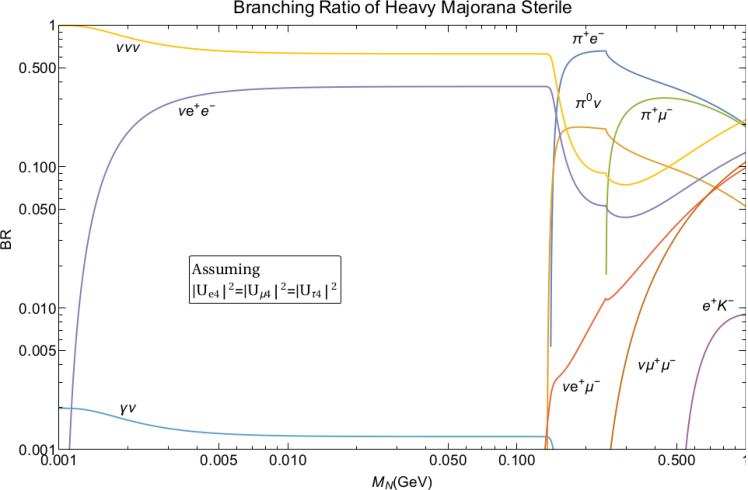
\includegraphics[width=0.8\textwidth]{figures/bounds1.pdf}\\
%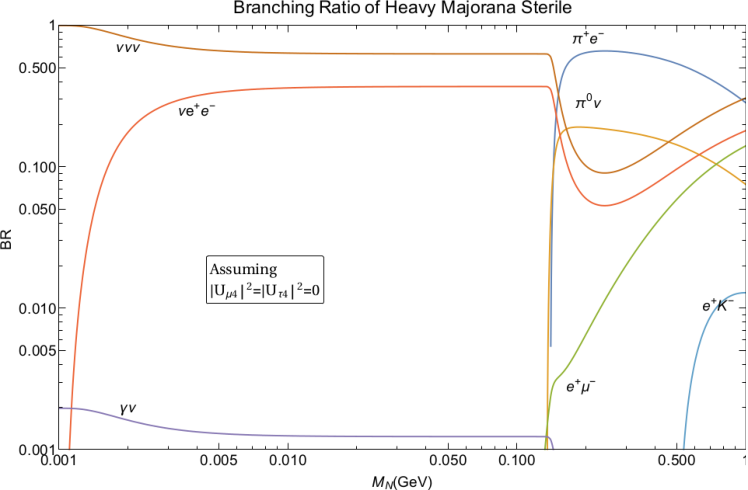
\includegraphics[width=0.49\textwidth]{figures/bounds2.pdf}
%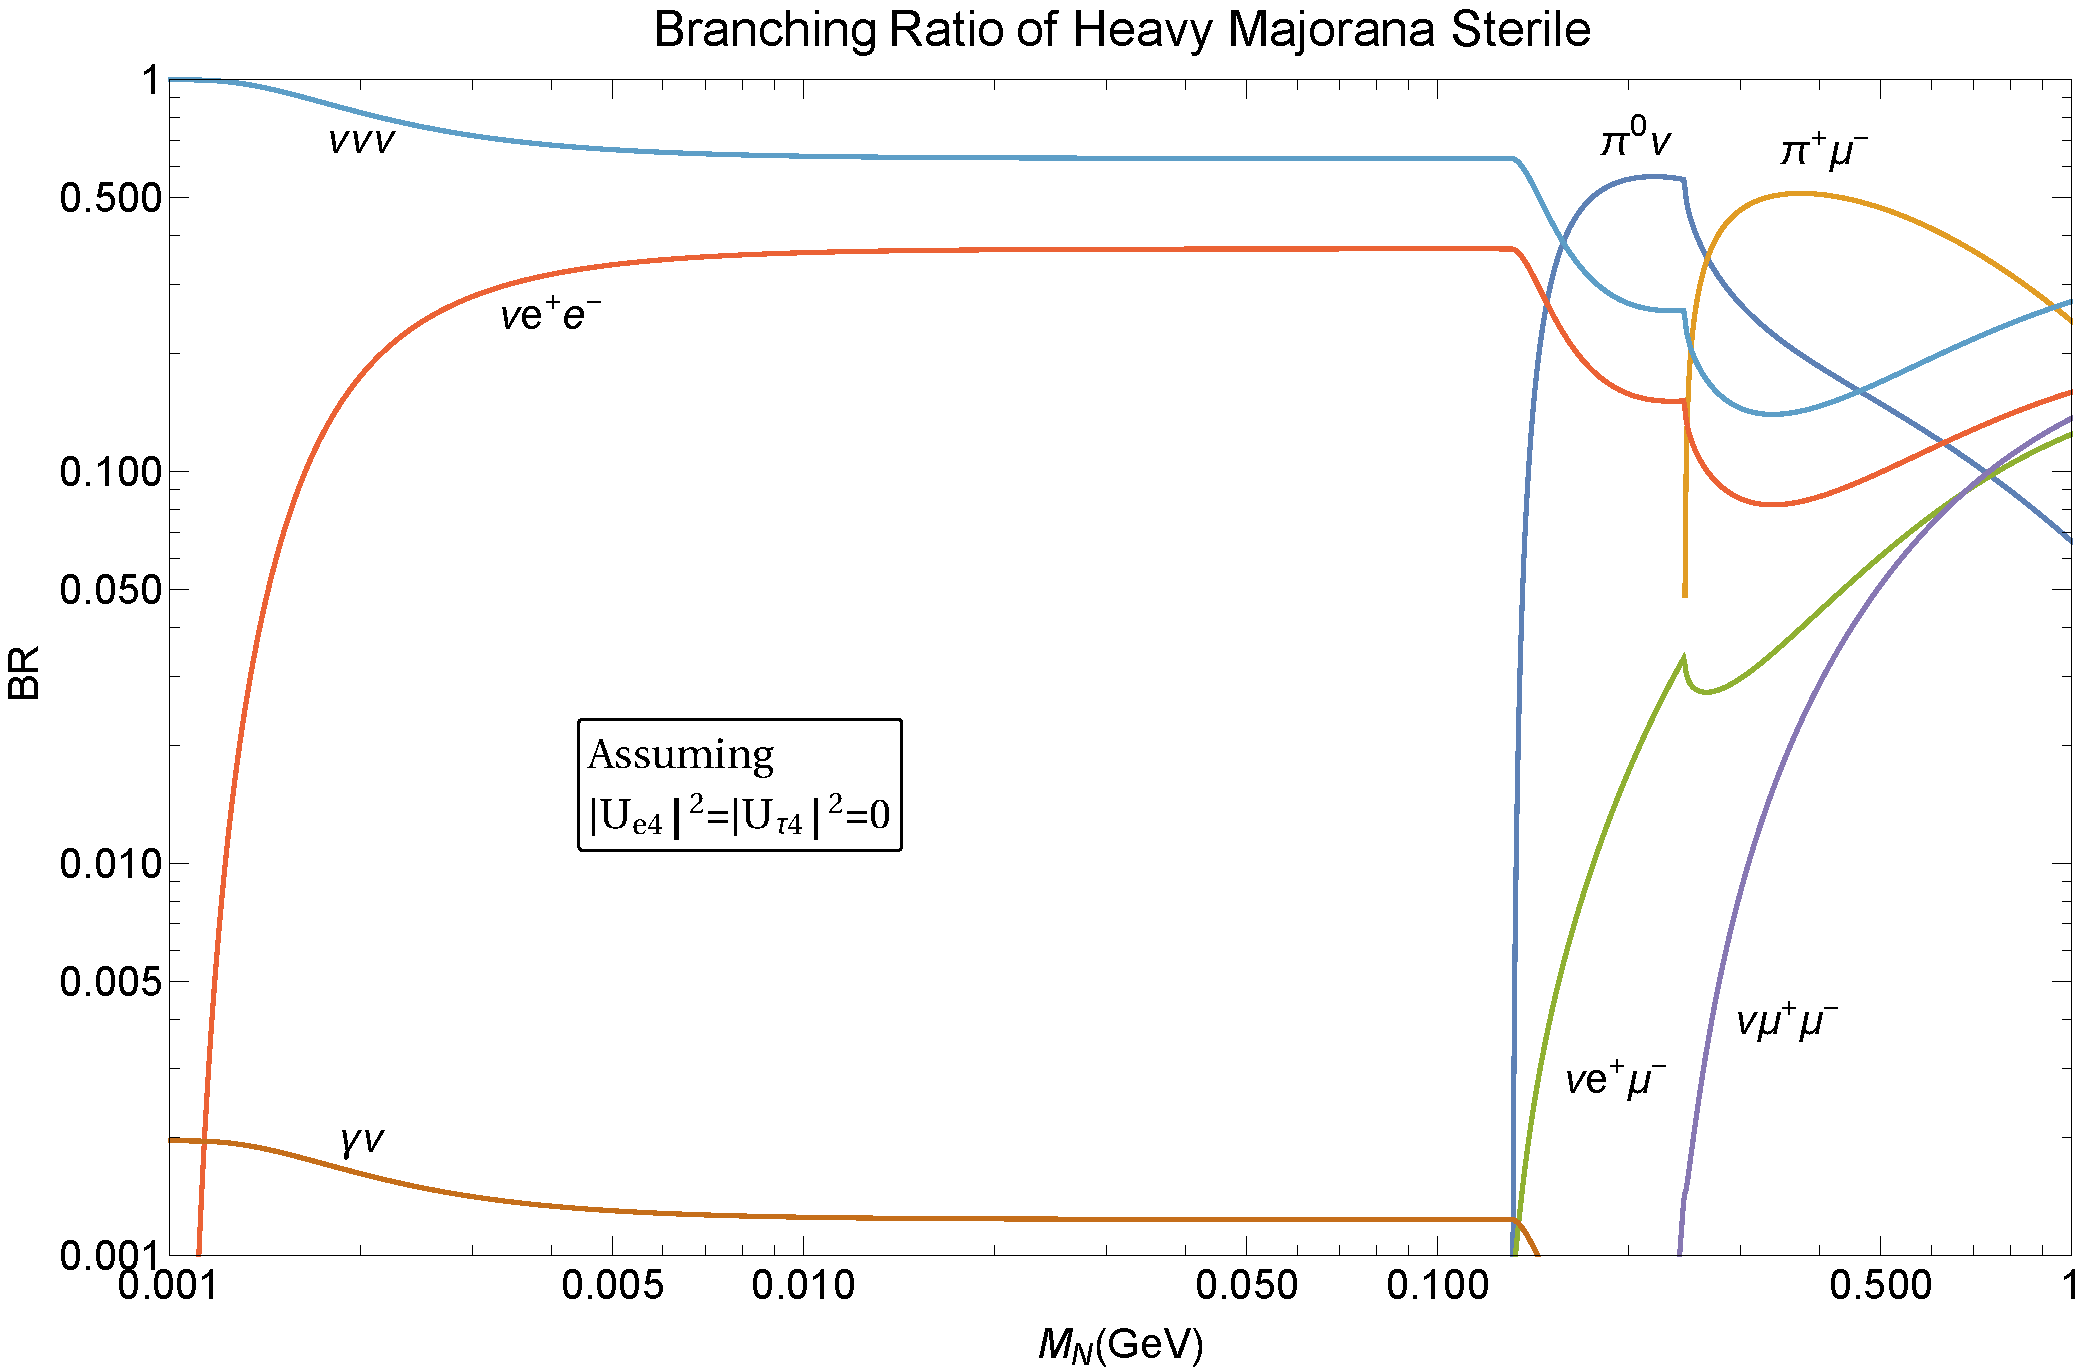
\includegraphics[width=0.49\textwidth]{figures/bounds4.pdf}
%
\caption{\label{fig:branchingratios}The branching ratios for sterile neutrino
decays in the minimal 3 sterile SM extension, with masses between 1 MeV and 1 GeV. This assumes equal
mixing with all active flavours. Note that below 100 MeV, $\nu_N \rightarrow \nu_\alpha e^+ e^-$ is by far the most dominant visible decay.\newtext{MARK}{Hmm, can put some nice information in big blank spot. but what?}}
%
\end{figure}

\subsection{Decays of interest}


We focus on five decays in our study, which have the largest branching ratios
of all channels with visible decay products over the mass range $m_\text{s}
\lesssim 1$ GeV. This is based on the minimal sterile extension of the SM
discussed above, and the discussion in this chapter will assume this model.
However, as discussed further in \refsec{sec:BMM}, we point out that similar
decays can also occur in non-minimal models, where the relationship between
decay rate, mass and mixing can be non-standard. 
%
For sterile neutrino masses less than the pion mass, the dominant visible decay
will be into an electron-positron pair as can be seen from
\reffig{fig:branchingratios}. This is true regardless of the flavour structure
of the mixing matrix. The decay rate for this channel is given by 
%
\[ \Gamma\left(\nu_\text{s}\to \nu_i e^+e^-\right) =
\frac{G_\text{F}^2m_\text{s}^5}{96\pi^3}I_1\left(0,\frac{m_e}{m_\text{s}},\frac{ m_e}{m_\text{s}}\right).  \]
%
where 
\begin{align}
	I_1(x,y,z) & =12 \int_{(x+y)^2}^{(1-z)^2} \frac{ds}{s}(s-x^2-y^2)(1+z^2-s)\sqrt{\lambda(s,x^2,y^2)}\sqrt{\lambda(1,s,z^2)},\\
\lambda(a,b,c) &= a^2+b^2+c^2 - 2ab-2bc-2ca.
\end{align}

%
Decays of this type would generally fall into two categories of events at a LAr
detector, and accordingly we divide our analysis. The first event sample will
attempt to measure events where two tracks are resolved and two
electron-induced electromagnetic showers are observed.
%
The second sample consists of events for which the identification of two
elecron-like showers is impossible. In this case, the signal would be identical
to a single photon pair-conversion. We expect a larger background for this
scenario, but as we will show, we get sizable event numbers in this channel due
to the sterile neutrino's high energy, and a tight cut on the angular
distribution can make it sensitive to sterile decays.

Also possible at these low masses, the radiative decay
$\nu_\text{s}\to\nu_i\gamma$ would generate an interesting single photon
signal \cite{PhysRevD.25.766}. In the minimal model the decay rate goes as
%
\[ \Gamma(\nu_\text{s}\to\nu_i\gamma) = \frac{G_\text{F}^2m_\text{s}^5 |U_{\alpha 4}|^2}{192 \pi^3} \left( \frac{27 \alpha}{32 \pi} \right), \]
%
this decay channel will be very small and the total decay rate can be estimated
at around $\Gamma(\nu_\text{s}\to\nu_i\gamma)/(\text{GeV}) \approx 10^{-20}
(m_\text{s}/\text{GeV})^5$, which could not be expected to be observable at
SBN.  However, in a non-minimal model this decay rate could be enhanced. For
example, such an enhancement has been proposed to resolve the MiniBooNE anomaly
\cite{Gninenko:2009ks,Gninenko:2010pr}.  

When the mass of the sterile neutrino is greater than the kinematic threshold
for the production of a neutral pion, a new decay dominates
$\nu_\text{s}\to\nu_i \pi^0$. The decay rate for this process is given by
%
\[ \Gamma\left(\nu_\text{s} \to \nu_i \pi^0\right) =
\frac{G_\text{F}^2f_\pi^2m_\text{s}^3}{64\pi} \left[1-\left(
\frac{m_\pi}{m_\text{s}} \right)^2\right].  \]

The next channel appears at the kinematic threshold for charged pion production
with a charged lepton. If mixing between the heavy mass state and the electron
neutrino is present, this decay occurs almost immediately after the $\nu\pi^0$
channel opens. However, if this mixing is negligible, there is a gap the size of
the muon mass before the $\mu^\pm\pi^\mp$ channel opens. As can be seen from
\reffig{fig:branchingratios}, these decays dominate the visible decays when
they are allowed. These decays have a similar scaling behaviour of the decay
rate to the $\nu\pi^0$ channel with an equivalent dependence on the pion
structure constant,
%
\[ \Gamma\left(\nu_\text{s} \to l^\pm\pi^\mp\right) =
	\left|U_{l4}\right|^2\frac{G_\text{F}^2f_\pi^2 |V_{ud}|^2  m_\text{s}^3}{16\pi}I\left(\frac{m_l^2}{m_\pi^2} , \frac{m_\text{s}^2}{m_\pi^2}\right) ,
\]
with 
\[
	I(x,y) = \left[ \left( 1+x+y\right) \left(1+x\right) -4 x\right] \lambda^\frac{1}{2}\left(1,x,y\right)
\]

As can be seen from Figure (\ref{fig:branchingratios}) there are several additional decays possible $\nu_s \rightarrow \nu_\alpha \mu^+ \mu^-$ and $\nu_s \rightarrow \nu_\alpha e^+ \mu^-$, however, in the kinematic region allowed under the assumption the steriles were produced in pion and kaon decays these channels have sub dominant branching ratios and are not included in this analysis.

\subsection{Non-minimal models of sterile decay}

All previous work assumed the minimal extension of one extra sterile degree of
freedom, with no additional physics such that the only decays allowed are
standard model weak processes with an active mixing scaling. 
%
In this model, all interactions of the mostly sterile mass state are produced
by neutrino mass mixing. If the fermion bilinears are removed from the
Lagrangian, the sterile decouples and all (non gravational) observable effects
vanish. An important feature of this model is the all or nothing approach to
decay rates: there is a single parameter, the mixing between the active states
and the mostly-sterile mass state, which dictates the magnitude of all the
decay rates. This is a great asset when trying to constrain the  minimal model,
for example it allows us to place bounds on the observation of $N\to \pi^0 \nu$
despite no experiment to-date reporting the results of such a search. 
%
While this model is minimal in it assumes no new fields or dynamics beyond the
single particle added at observable scales and its renormalizable interactions,
there is no theoretically appealing mechanism to explain a neutral fermion with
a mass below the electroweak scale as well as the sizes of neutrino masses
without the presence of heavier fields in the neutrino sector. The natural
consequence of decoupling these heavy particles would be to generate
non-renormalizable operators which allow for a richer phenomenology for the
intermediate scale sterile than the terms in the minimal extension. Therefore it 
seems relevant to consider models where the minimal interactions produced by 
mass-mixing are supplemented by other operators leading to potentially 
higher decay rates.

In this scenario, the minimal couplings are always present. Therefore, without
suspicious cancellations between the mixing-derived and higher-dimensional
contributions to a decay, the non-observation of a signal in a given decay
channel tells us that the event rate is less than or equal to the bound
produced in the minimal model. The process may still be driven by new physics,
and accordingly we would interpret the factor $U^2$ differently, but the total
rate is bounded in a robust way. However, in the most general extension of the
$\nu$SM we must allow for some decays to be enhanced to a greater extent than
others. This could break the correlation between decay rates present in the
minimal model, and in the case that we are using one channel \emph{e.g.} $N\to
e^+e^-$ to bound another which has not been directly constrained \emph{e.g.}
$N\to\nu\pi^0$, the bounds on the unobserved channel are potentially violated 
and detectable signals could be present.

For the reasons discussed so far, we believe it is relevant to place bounds on
the possible decays of a neutral fermion in an extended scheme which allows for
arbitrary decay rates to visible particles (within the bounds of perturbativity
and other conventional model building constraints).
%
In this section we will consider the possibility of enlarged neutral current
decay rates for the mostly-sterile fermion. In this scenario, the production of
the novel fermion will be largely unaffected by the new physics: heavy states
will be produced in the beam from meson decay via the flavour off-diagonal
charged current interactions as usual. However, we allow for an arbitrary rate
of decay for the three channels
%
\[  \Gamma_{\gamma\nu},\qquad \Gamma_{e^+e^-}\qquad \text{and} \qquad
\Gamma_{\pi^0\nu}. \]
%
 When considering enlarged decay rates, we must be careful with existing bounds
on the model, as an enlarged decay rate would affect all prior beam dump
experiments in the same way until the point where baseline dependence becomes
significant. 

\section{\label{sec:timing}Role of event timing}


\begin{figure}[t]
%
\center
%
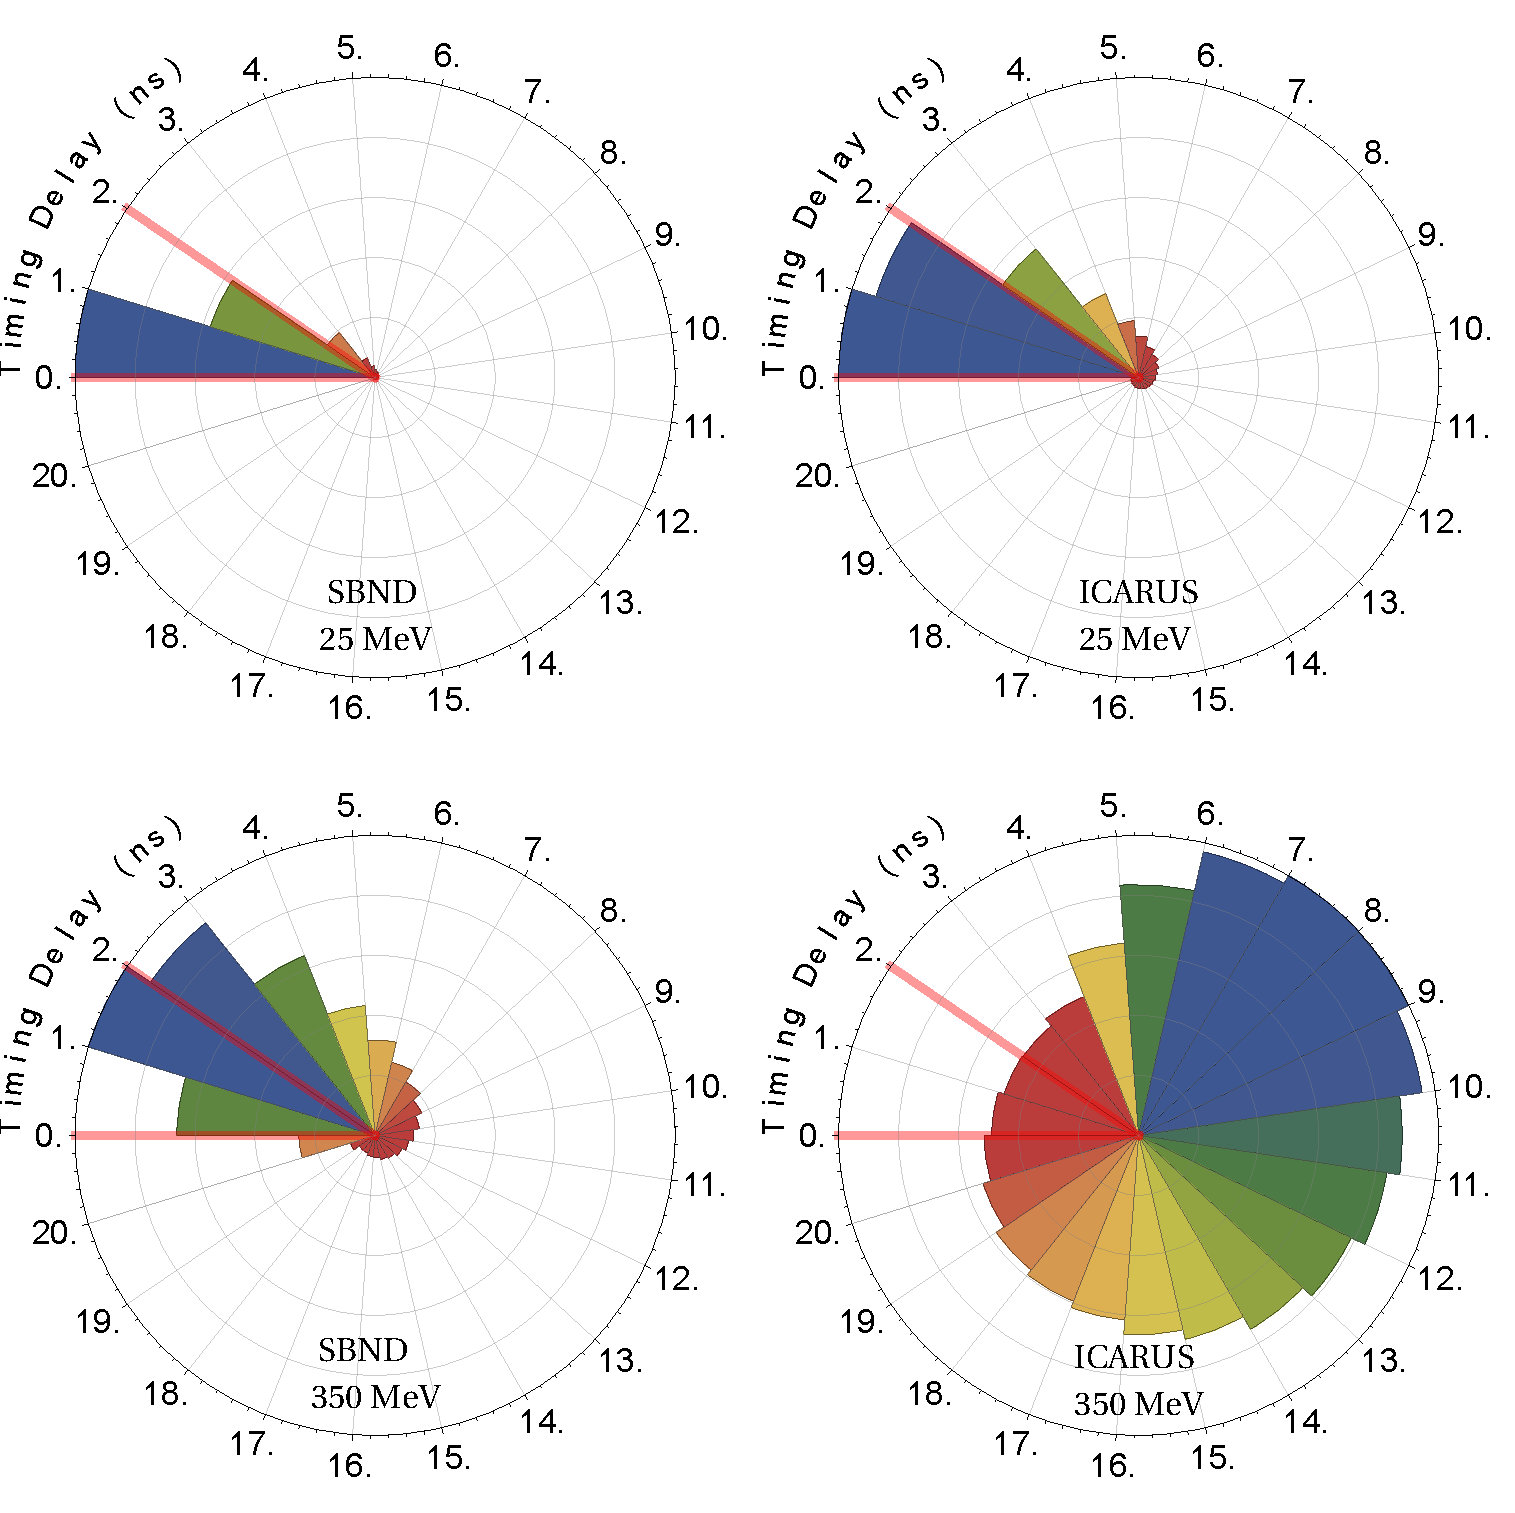
\includegraphics[width=0.75\textwidth]{figures/timing.pdf}
%
\caption{\label{fig:timing} Shown above is the timing delay of sterile neutrino
decays in nano-seconds for both a 25 MeV (top) and 350 MeV (bottom) sterile
neutrino at the SBND and and Icarus detectors (110 and 600m
respectively). The 2 ns beam bucket window is shown highlighted in red from 0
to 2 ns, followed by an additional 19 ns gap. The timings are calculated as a
difference to the time of flight of a active neutrino, assuming the decay
occured in a uniform sample accross the 50m BNB decay pipe. A timing resolution
of 1 ns is assumed to smear the observed events.}
%
\end{figure}

One of the interesting features of the SBN complex is the interplay of the
three detectors, operating similar technology but situated at different
baseline distances.
%
Light neutrinos reach the furthest detector of the SBN complex after around 2
$\mu$s; however, sterile neutrinos of MeV-scale masses can move considerably
slower as their mass gets larger. For a very boosted sterile, this difference
is small and no observable effects arise. When the sterile becomes less
boosted, however, the timing structure of the BNB becomes relevant.

In the conventional physics programme of the SBN, timing plays an important
role in the analysis of backgrounds, tight timing windows are placed around the
beam spill to limit constant rate backgrounds such as cosmogenic events. The
BNB consists of 81 Radio-Frequency buckets of approximately 2ns length,
seperated by 19 ns, to form a 19.2$\mu$s spill with a frequency of 3Hz
\cite{Antonello:2015ea}.  All events inside this window, alongside all events
in the surrounding bins according to assumed resolution, are assumed to be
beam-correlated.  As can be seen in \ref{fig:timing} below, for sterile masses
around $25$ MeV, most decay events will end up in the beam timing window and
must be analysed as a signal on top of the beam-related backgrounds in the
standard analysis. However, as the sterile neutrino mass incresaes, the
baseline distance starts to become relevant. At $m_{\text{s}}=350$ MeV, we see
that many events still fall in the in beam timing window for SBND; however,
\muboone\ and Icarus see significant deviation from this with clear peaks in
the inter-RF-bucket spacing where one would not expect to see any
beam-correlated backgrounds. Events falling outside these bins, would not be
counted as part of the beam-related event sample. Assuming the backgrounds can
be brought under control in these different timing windows, this signature
would be a striking one: a beam-related excess at SBND with none at \muboone\
or Icarus, but an excess at both sites in their non-beam related data.

The implication of the timing effects, is that our discussion of backgrounds
must be divided in two cases: for low mass steriles or any mass at SBND, we
must consider the beam-related backgrounds and see how these can be suppressed
to enhance the significance of the signal events. For larger masses at the two
furthest detectors, we must instead consider how to isolate our signal events
from the non-beam related background, made predominately from cosmogenic
events. In the section that follows we will discuss the details of our signal
modelling and background estimation, and compute the sensitivities to new
physics in \refsec{sec:sensitivity} including a discussion of the 
use of timing and baseline distance in \refsec{sec:baselineinterplay}. 

\section{Simulation details}

We have computed the fluxes and simulated event numbers for each beam and
detector via a custom Monte Carlo program. The program allows efficiency's to
be taken into account due to experimental details of the detector and its
capabilities in a fully correlated way between observables. 

The fluxes from BNB are taken from REF, and we assume no spectral modifications
associated with the altered kinematics of the new sterile neutrino final state.
%
Given the spectral flux of sterile neutrinos in the BNB,
$\mathrm{d}\phi/\mathrm{d}E$, we compute the total number of accepted events in
channel ``$\text{c}$'' via the following summation,
%
\[ N_\text{c} = \sum_{i} \left .
\frac{\mathrm{d}\phi}{\mathrm{d}E}\right|_{E_i} P_\text{D}\left(E_i\right)
W_\text{c}\left(E_i\right),  \]
%
where $P_\text{D}(E)$ is the probability for a sterile of that energy to reach
and then decay inside the detector labelled $\text{D}$. The simplest
approximation is to ignore all geometric effects, so that every particle
travels exactly along the direction of the beam line, which gives the following
probability 
%
\[ P_\text{D}\left(E\right) = e^{-\frac{\Gamma_\text{T}L}{\gamma\beta}}\left(
1-
e^{-\frac{\Gamma_\text{T}\lambda}{\gamma\beta}}\right)\frac{\Gamma_\text{c}}{\Gamma_\text{T}},
\label{eq:prob}
\]
%
where $\Gamma_\text{T}$ ($\Gamma_\text{c}$) denotes the rest-frame total decay
width (decay width into channel $\text{c}$), $m$ the mass of the sterile
neutrino, and $L$ ($\lambda$) the distance to (width of) the detector. The
combination $\gamma\beta$ is the usual special relativistic function of
velocities of the parent particle and provides the sole energy dependence of
the expression
%
\[   \frac{1}{\gamma\beta} \equiv \frac{m}{\sqrt{E^2-m^2}}. \]
%
As we are exploring a large parameter space, often this expression takes a
simplified form depending on the size of $\Gamma_\text{T}\lambda/\gamma\beta$:
%
\begin{align*} 
%
\Gamma_\text{T}\lambda \ll 1\qquad&\qquad P_\text{D} \approx
e^{-\frac{\Gamma_\text{T}L}{\gamma\beta}}\frac{\Gamma_\text{c}\lambda}{\gamma\beta}
+ \mathcal{O}\left(\Gamma_\text{T}^2\lambda^2\right),\\ 
%
\Gamma_\text{T}\lambda \gg 1\qquad&\qquad P_\text{D} \approx
e^{-\frac{\Gamma_\text{T}L}{\gamma\beta}}\frac{\Gamma_\text{c}}{\Gamma_\text{T}}
+ \mathcal{O}\left(\frac{1}{\Gamma_\text{T}\lambda}\right), 
%
\end{align*}
%
where the rate for slowly decaying particles can be seen to grow with detector
size until a width of $\lambda\sim\Gamma_\text{c}^{-1}$ where longer detectors
make no difference, as most steriles decay within a few decay lengths and
therefore we see a fixed fraction of the total events in our channel of interest. 
We will comment on how the three detectors of the SBN complex can use the 
dependence on $E$ and $L$ in these expressions to enhance their sensitivity in 
Section ??.

%
Finally, the function $W_\text{c}(E)$ is a weighting factor which accounts for
all effects which reduce the number of events in the sample: for example,
analysis cuts or detector performance effects.
%
To compute these factors, we run a Monte Carlo simulation of the decays for a
large number of sample events with a given energy. Each sterile event is
associated with a decay of type $\text{c}$. We then apply experimental analysis
cuts to the decays based on our assumptions about the detector's capabilities
and backgrounds, to produce a spectrum representing the final event sample. The
percentage of accepted events defines the weight factor for that energy.

We alsod work spectrally producing the expected distributions of observed
events. This can be used to suggest improved analysis cuts based on the
interplay between the three detectors of the SBN complex. We return to this in
section II.

\subsection{Sterile neutrino fluxes}

To leading order in the mass of the sterile neutrino over the pion, the fluxes
for the $\nu_\text{s}$ will be a rescaling of the fluxes for the active
neutrinos.  We take these fluxes as our input and scale them by the appropriate mixing $U_{\alpha 4}$, with an additional kinematic factor to take into account the helicity un-suppression of channels such as $\pi^+ \rightarrow e^+\nu_s$ for massive $\nu_s \gg m_e$. The flux of steriles produced from the decay of a meson M is therefore given by
\[
	\phi_{\nu_s}(E_{\nu_s}) \approx \phi_{\nu_\alpha} (E_{\nu_\alpha})\vert U_{\alpha 4}\vert^2 \frac{\rho\left( \delta_M^a , \delta_M^i \right)}{\delta_M^a \left(1- \delta_M^a\right)^2}.
\]
Where $\rho(a,b)=\mathcal{F}_M(a,b) \lambda^{\frac{1}{2}}(1,a,b)$ is a kinematic factor consisting of a term proportional to the two body phase space factor, $\lambda(x,y,z)=x^2+y^2+z^2-2(x y+yz+x z)$ and a term proportional to the matrix element, $\mathcal{F}_M(a,b)= a+b -\left(a-b\right)^2$, with $\delta_M^{a(i)}=m_{l_a(\nu_i)}^2/M^2$ \cite{PhysRevD.24.1232}. This kinematic effect for the pion and kaon, the only mesons produced in large numbers in the BNB beam, is shown below in figure \ref{fig:flux_enhancement}. We only consider steriles below the kinematic threshold of the kaon (388 MeV for $|U_{\mu4}|$ production and 493 MeV for $|U_{e4}|$ driven production) as although there is a small component of heavier mesons such as the D meson which could produce heavier sterile states, they are produced in very small numbers due to the relatively low energy protons of the BNB beam. As the mass of the sterile increases, we begin to see componants of the flux having energies less that the sterile mass, artifically loosing these events. In order to keep the normalisation of total neutrino events constant, before $U_{\alpha 4}$ and kinematic scaling, these events are shifted to be above the sterile mass threshold. \\

The neutrino fluxes at all three SBN detectors are calculated from published MiniBooNE fluxes \cite{AguilarArevalo:2008yp}, after scaling by appropiate $1/r^2$ baseline dependance, e.g $(470/540)^2 \approx 1.3$ at $\mu$BooNE. This is similarly scaled by $1/r^2$ for ICARUS at 600m, however, an additional energy dependant flux modifier is applied for SBND at 110m to account for the softer energy spectrum due to the proximity of the detector to the production target \cite{Antonello:2015lea}. We consider sources of neutrinos that are dominant in at least one energy range including wrong sign neutrinos, smaller subdominant $K^+\rightarrow \pi^+\rightarrow \nu_\alpha$ as well as other contributions, predominitely from meson decay chains initiated by meson-nucleus interactions, although all contributions other than neutrinos from two body meson decays are scaled by $|U_{\alpha 4}|^2$ only, not including the kinematic enhancement mentioned above. The neutrino spectrum at $\mu$BooNE is shown below in figure (\ref{fig:nuflux}). 

\begin{figure}[t]
\center
\begin{subfigure}[t]{0.5\textwidth}
	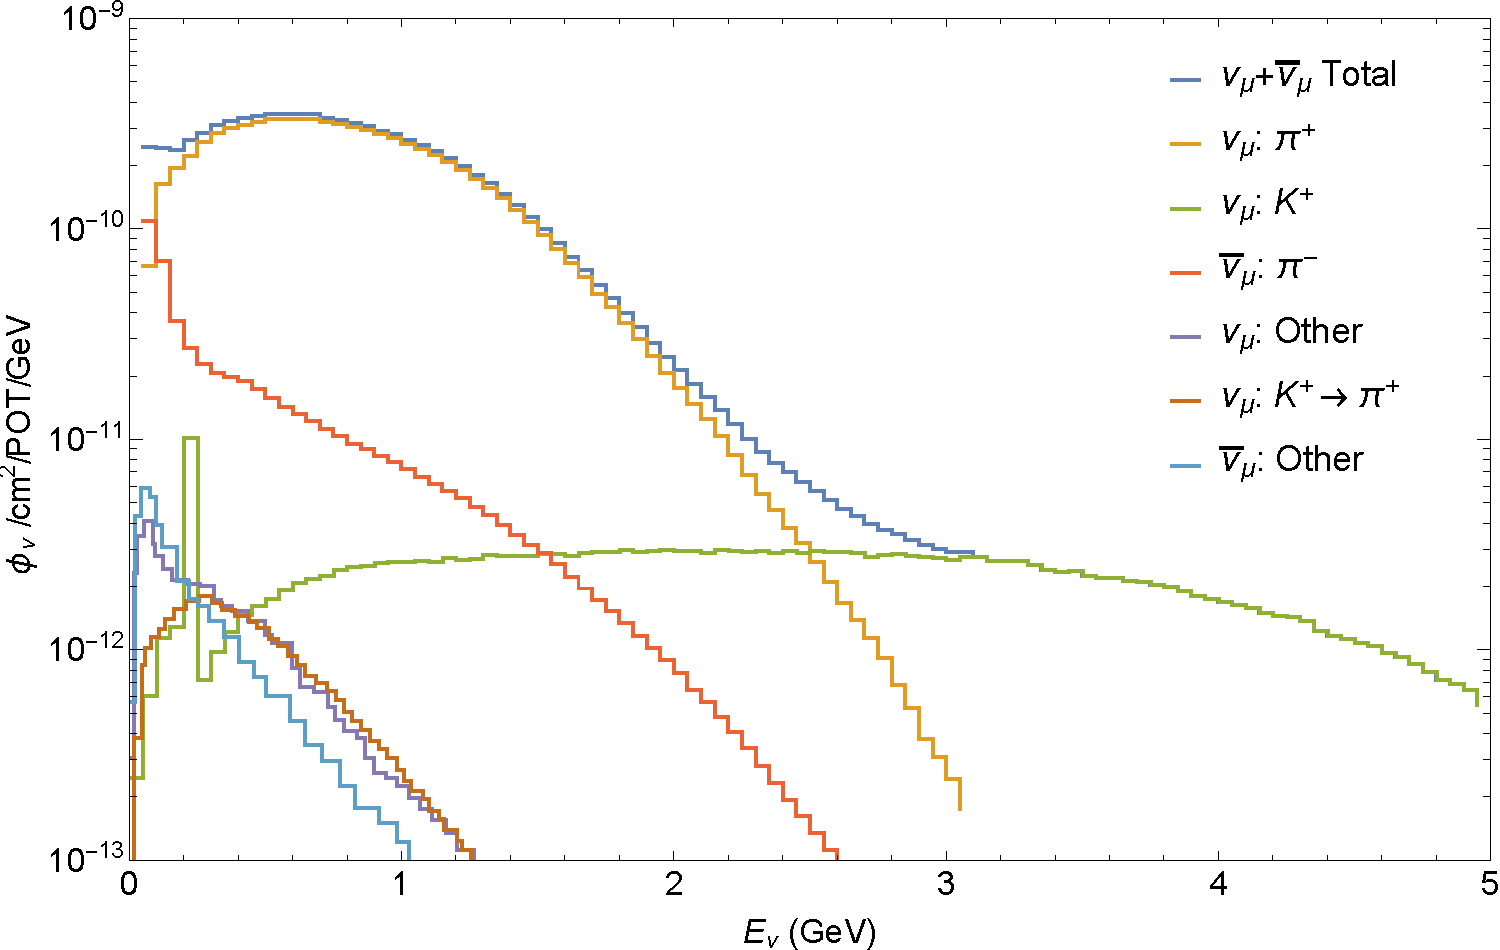
\includegraphics[width=\textwidth]{figures/microBooNE_flux.pdf} 
\end{subfigure}%
~
\begin{subfigure}[t]{0.5\textwidth}
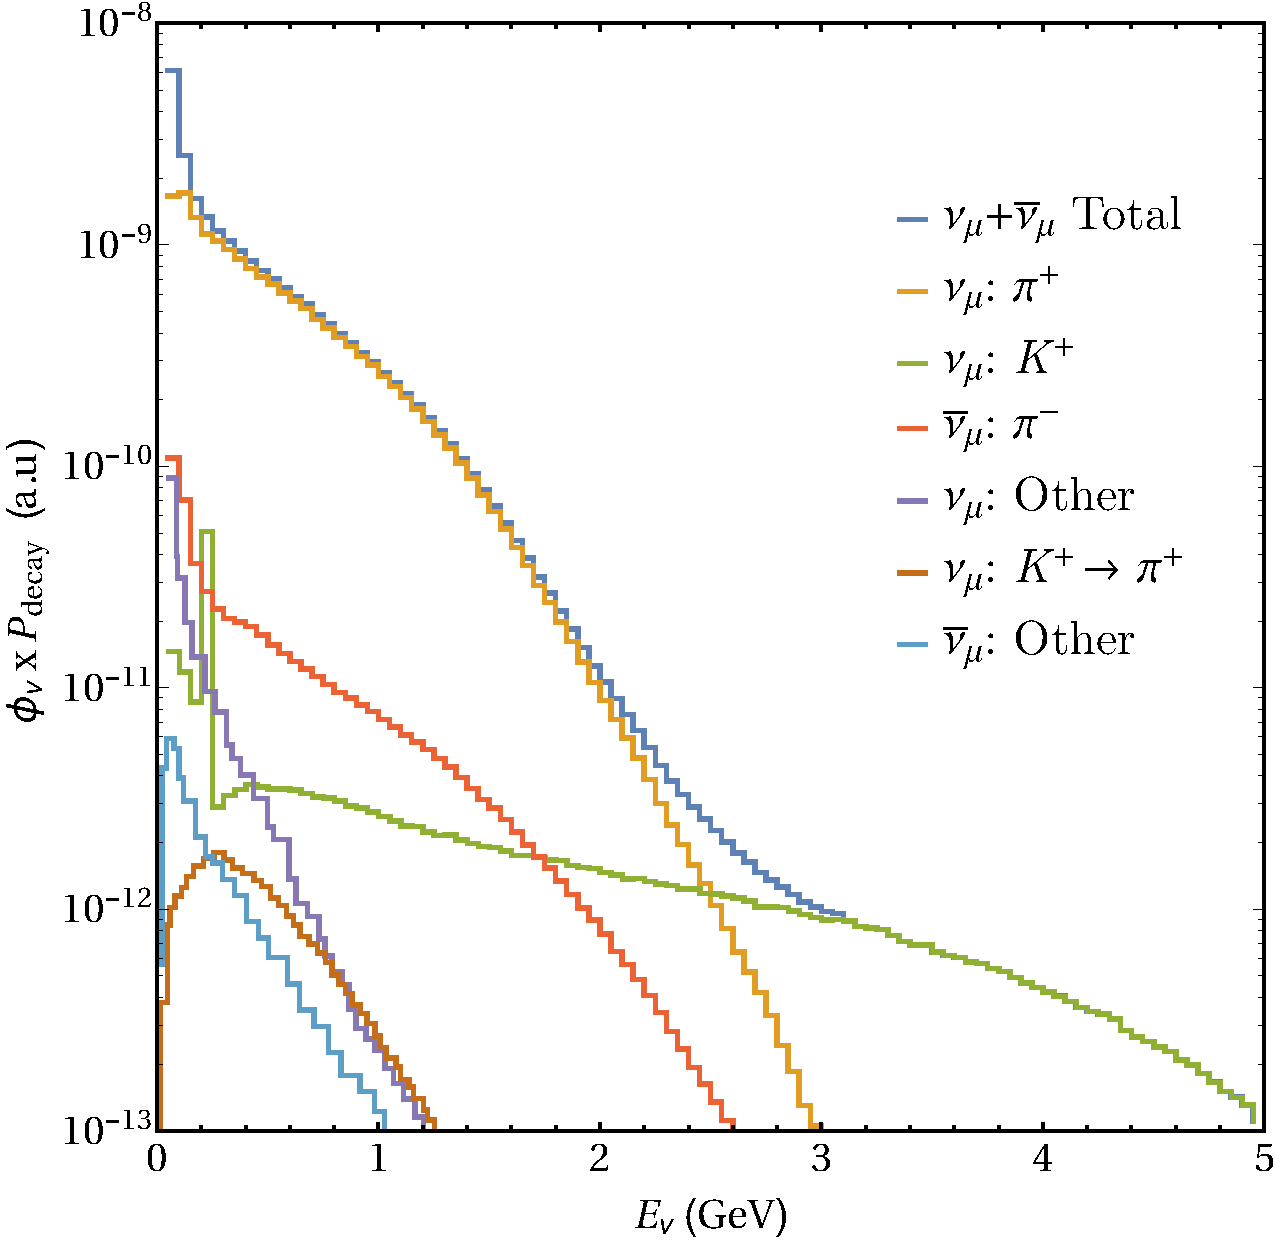
\includegraphics[width=\textwidth]{figures/microBooNE_flux_weighted.pdf}
\end{subfigure}
\caption{\label{fig:flux_plots} Left: The composition of fluxes of $\nu_\mu$ and $\overline{\nu}_\mu$ at $\mu$BooNE with horn in positive polarity (neutrino mode). ``Other'' refers to contributions primarily from meson decay chains initiated by meson-nucleus interactions. Right: Fluxes weighted by the probability to decay inside \muboone, for a sample 25 MeV sterile with equal $|U_{e4}|^2 = |U_{\mu 4}|^2$, and the horn in neutrino-mode. Requiring that the sterile decays has the effect of vastly increasing the importance of lower energy bins. }

\end{figure}

\begin{figure}[t]
\center
	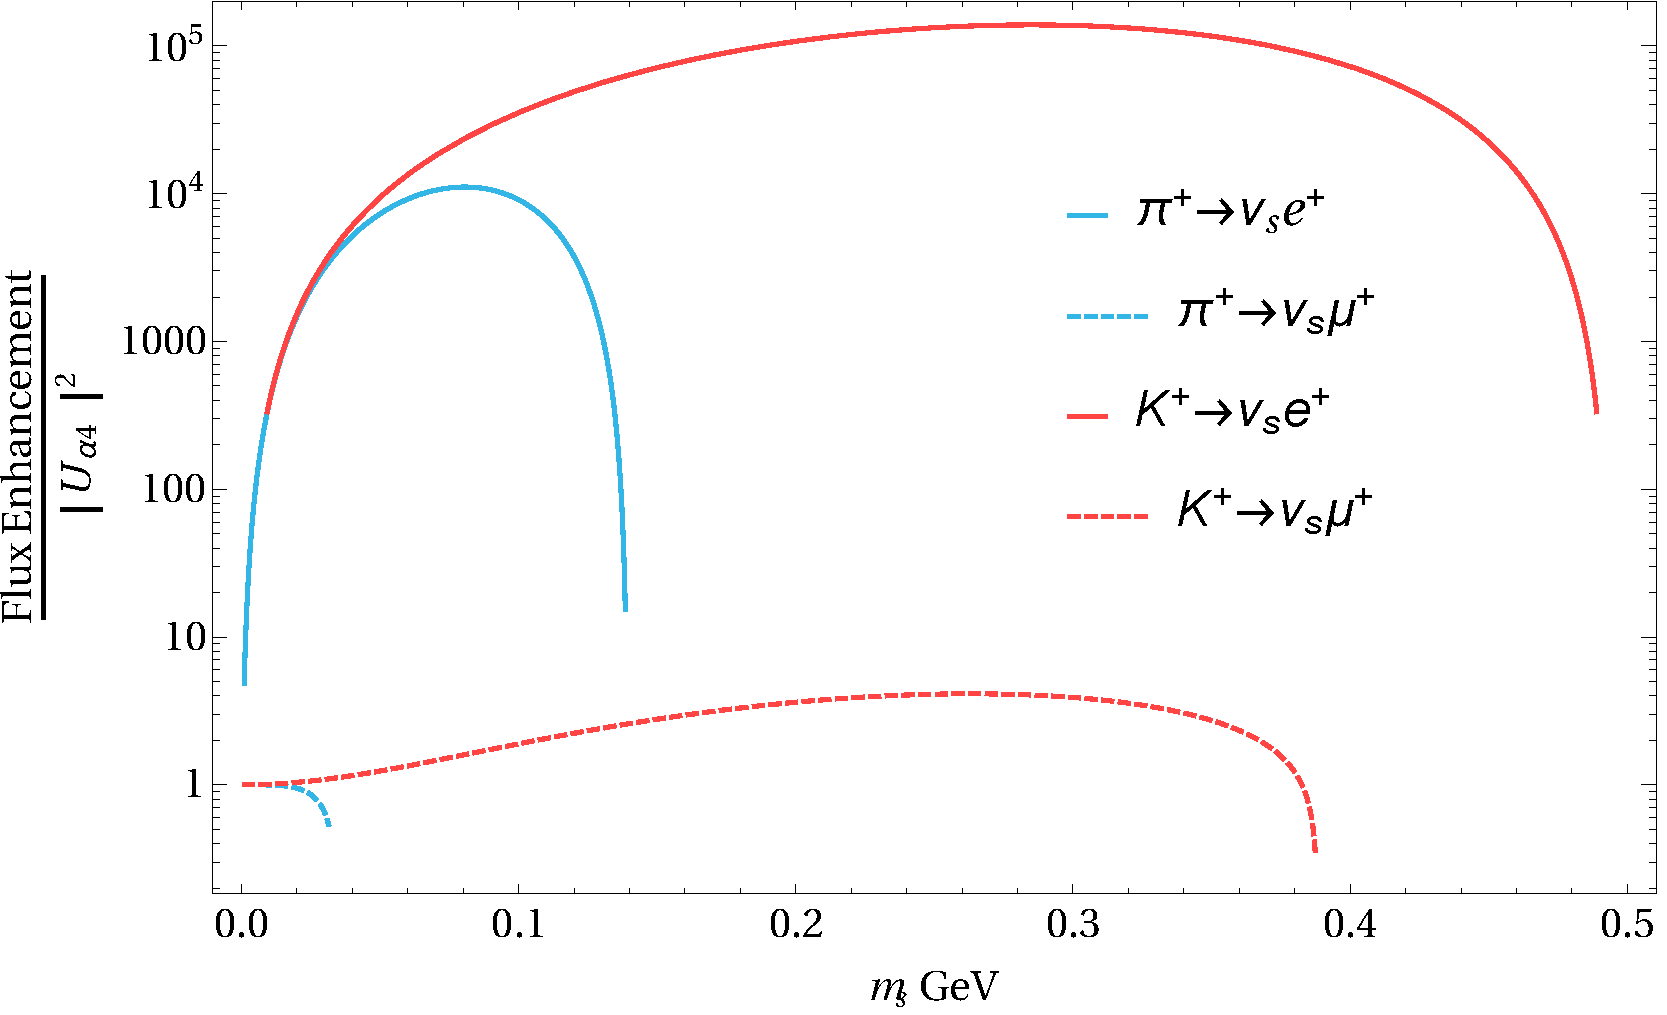
\includegraphics[width=0.6\textwidth]{figures/BNB_flux_enhancement.pdf} 
\caption{\label{fig:flux_enhancement}Kinematic enhancements of the sterile flux, for the four production channels available for steriles in the BNB beam. There is little effect when mixing with muons alone, as the muon is heavy enough to remove the helicity suppression that usually kills the $\pi\rightarrow e \nu$ channels. This factor of up to $10^5$ enhancement more than compensates for the significantly smaller flux of $\nu_e$ always inherent in the BNB beam.}

\end{figure}


%\subsection{Reproducing PS-191}
As a consistency check of our methodology, we reproduce in \reffig{ps191test}
the published bounds of PS-191. The detector geometry is assumed to be
$6\text{m} \times 3\text{m} \times 12 \text{m}$ and was located 128m downstream
of the Beryllium target using 19.2 GeV protons from the PS proton beam.  Fluxes
of all neutrinos produced from pion sources at PS-191 were obtined from
\cite{ps191THesis}. No accurate kaon sources could be obtained and as such only
low mass bounds are reproduced here. It must be noted that PS-191 ignored all
neutral current contribtions to $\nu_N \rightarrow \nu_\alpha e^+ e^-$ and
assumed the sterile neutrinos were Dirac particles; the effective of this is
that the bounds are not directly comparable to the minimal model discussed
above.


\begin{figure}
\center
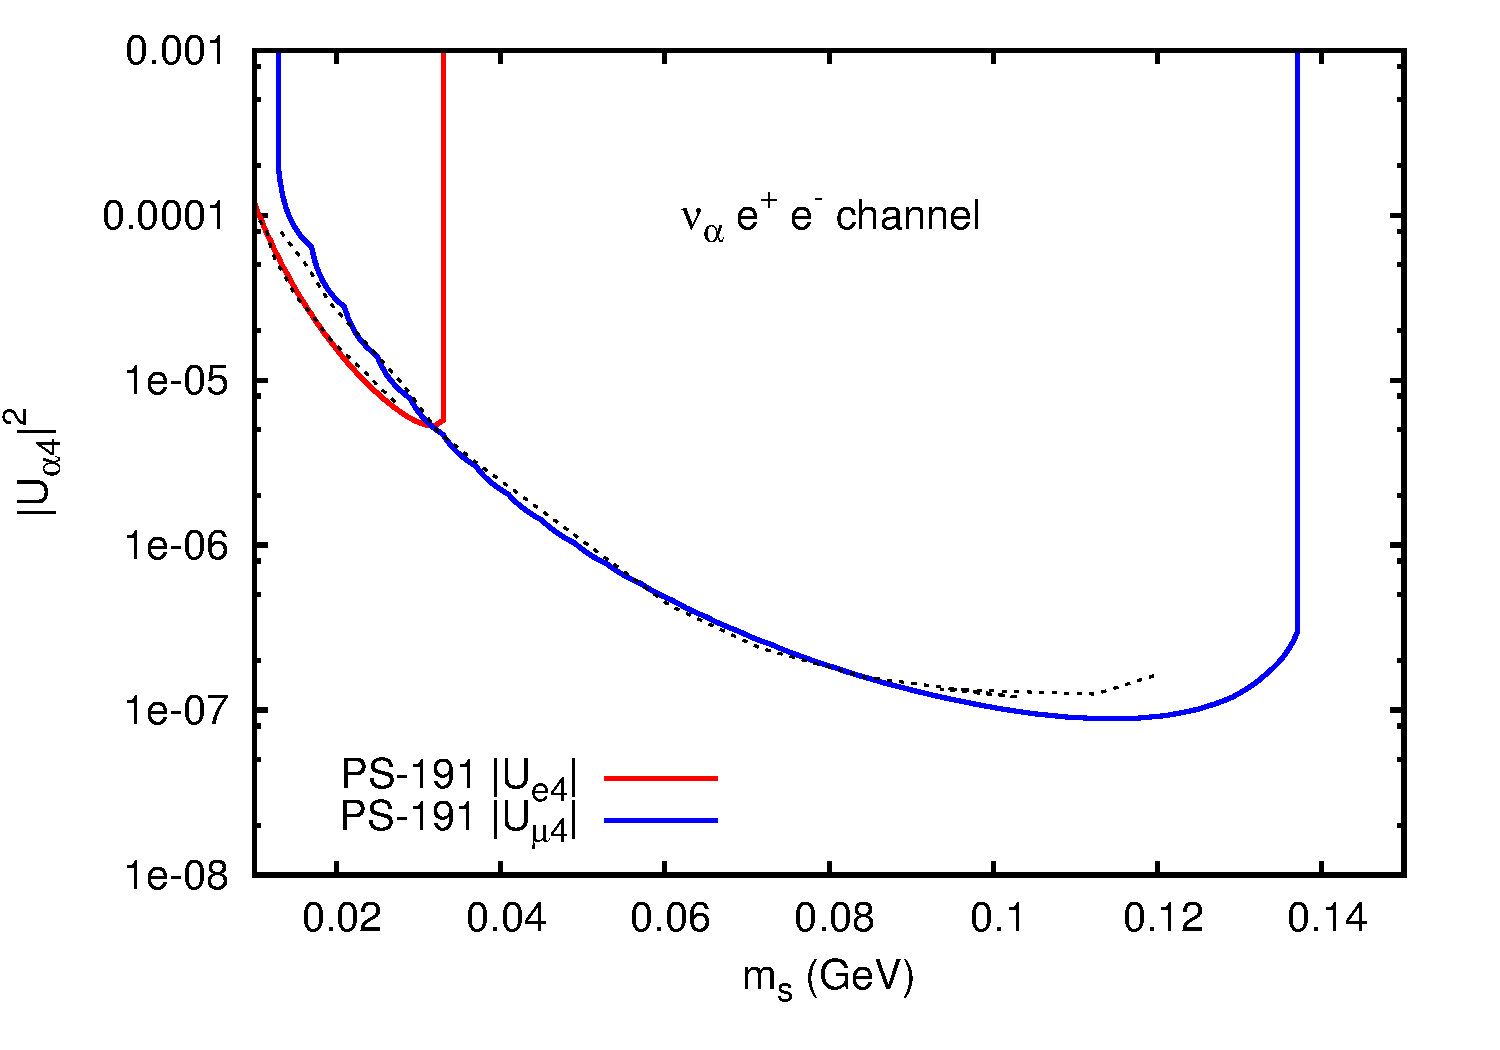
\includegraphics[width=0.7\textwidth]{figures/PS-191_test.pdf}
\caption{\label{fig:ps191test} Estimated bounds on $|U_{e4}|^2$ and $|U_{\mu 4}|^2$ for a Dirac heavy sterile neutrino decaying to $\nu_\alpha e^+ e^-$ at PS-191. The dotted black lines are the 90\% C.L results as published by PS-191, and the blue and red curves are the results of our simulation for $0.86 \times 10^{19}$ POT.}
\end{figure}

\subsection{Detector modelling and analysis cuts}

To compute the weighting factors $W_\text{c}$, we generate a large number of
Monte Carlo events of the decay that we are interested in and remove those
events which fail a series of cuts. These cuts are designed to reflect both
genuine analysis cuts designed to enhance the signal to background ratio (for
example, choosing events with energies within certain ranges), as well as cuts
which provide a basic model of detector effects and limitations (for example,
discarding events that wouldn't be reconstructed correctly, \eg\ those with
overlapping tracks in a two particle final state).

We summarize our cuts in \reftab{tab:cuts}.
%

\subsection{Signal distributions}

\lorem\lorem 

%\newtext{PB}{We can compute all types of kinematic distributions to talk about
%cuts.} See \reffig{fig:ang_sep_E_total}.
%


%\begin{figure}[t]
%\center
%\includegraphics[width=1.0\textwidth,clip,trim=0 0 0 0]{figures/ang_sep_E_total_plot.pdf}
%
%\caption{\label{fig:ang_sep_E_total}The distribution of total energy deposited in an $e^+e^-$ pair from sterile neutrino decay in flight at \muboone\ against the apparent angular separation of the two particles.}
%
%\end{figure}
%
%
%\section{BNB Beam Timing}
%The above beam related backgrounds are relavent for lower mass steriles, $m_s \leq 50$ MeV and for highly boosted heavy steriles at SBND. Once the sterile becomes less boosted, however, the timing structure of the BNB becomes very relevant for which backgrounds dominate. The Booster neutrino beam consists of 81 Radio-Frequency(RF) buckets of approximately 2ns length, seperated by 19 ns, to form a 19.2$\mu$s spill with a frequency of 3Hz. All events inside this window, alongside all events in the surrounding bins according to an assumed 1ns resolution, are possibly beam-correlated. As can be seen in \ref{fig:timing} below, this is mainly true for light sterile neutrinos at all three SBN detectors, as well as a resonable approximation of heavy neutrino timings at SBND, however, $\mu$BooNE and ICARUS see significant deviation from this with clear peaks in the inter-RF-bucket spacing where one would not expect to see any beam-correlated backgrounds. \\
%
%Outside of the RF bucket timing window, where beam-driven backgrounds are relavant, one must have a very strong grasp of cosmogenics backgrounds. However, due to the high energy and very forwardness of the decay events, alongside the fact that one can observe the cosmogenic background in beam-off mode, gives us {\bf {\emph{faith}}} that one can get veyr close to backgroundless (Ya need to show this..). 
%
%The use of timing signals is significantly enhanced by the fact SBN has three detectors at varying baselines. If one observes an excess of events in SBND that appears consistant with a heavy sterile decaying in flight, this must correlate with a scaled number of events with an appropiate out-of bucket phase in both $\mu$BooNE and ICARUS. If this is not observed, one can rule out the decay in flight scenario.
%
%
%\begin{figure}[t]
%\center
%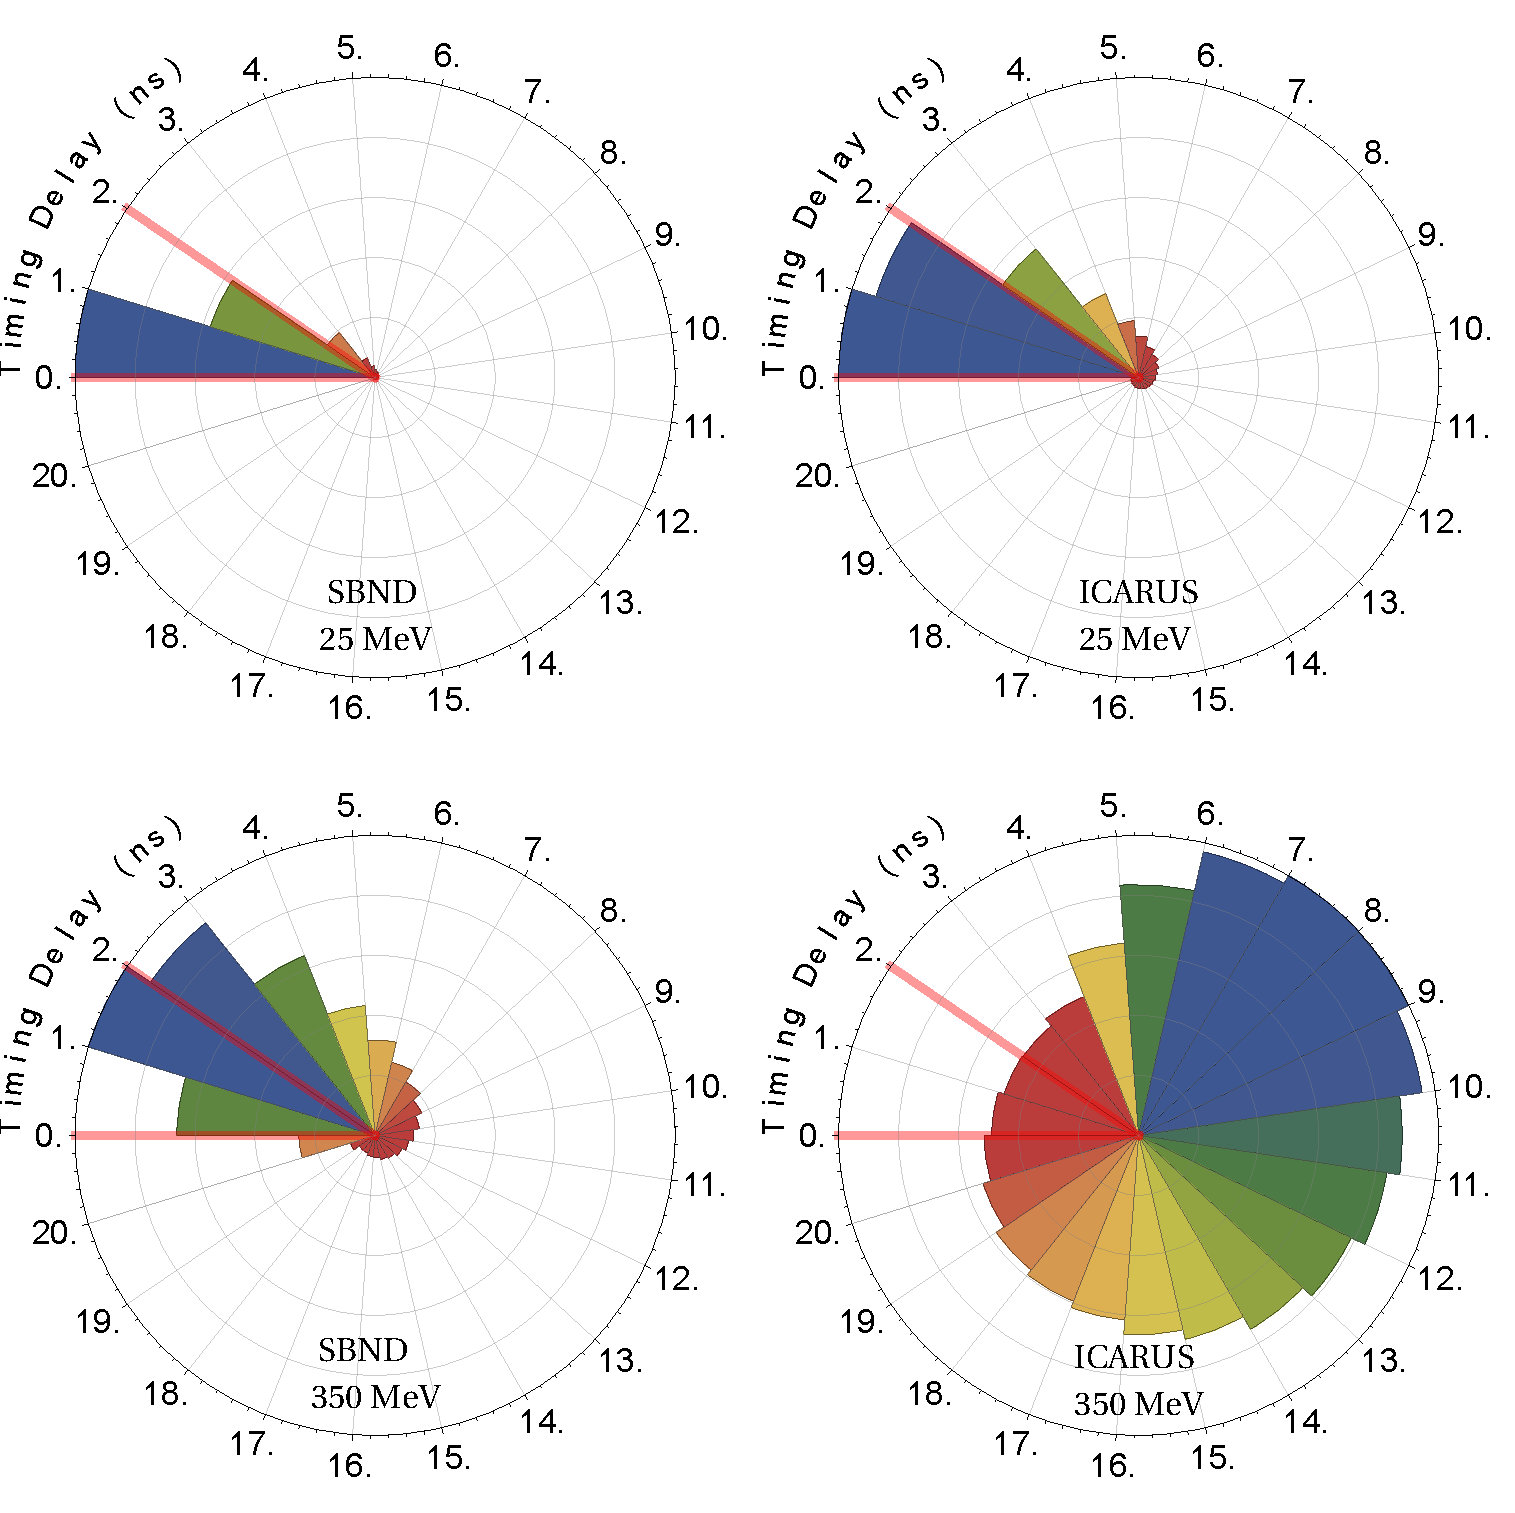
\includegraphics[width=\textwidth]{figures/timing.pdf}
%\caption{\label{fig:timing} Shown above is the timing delay of sterile neutrino decays in nano-seconds for both a 25 MeV (top) and 350 MeV (bottom) sterile neutrino at the SBND, $\mu$BooNE and ICARUS detectors (110,470 and 600m respectively). The 2 ns beam bucket window is shown highlighted in red from 0 to 2 ns, followed by an additional 19 ns gap. The timings are calculated as a difference relative to the time of flight of a active neutrino, assuming the decay occured in a uniform sample accross the 50m BNB decay pipe. A timing resolution of 1ns for all three SBN detectors is assumed to smear the observed events.}
%\end{figure}
%

\section{Sensitivities from total rate analysis\label{sec:sensitivity}}

The Fermilab SBN complex will be able to bound new physics models which lead to
sterile neutrino decay in the same manner as previous beam dump experiments: by
searching for anomalously high rates of specific decays. Searches of this kind
are usually done as total rate analyses, and the factor limiting the
performance  of the experiment is the total number of protons on target (POT).
In this section we consider the bounds that SBN can place on new physics
running in this mode, that is we assume that all events, regardless of their
timing information are collected into the same event sample. For SBND this is a
realistic model of the experiments operation: all of the heavy states
considered in this paper will generate decays in the normal event sample
associated with the neutrino beam. For \muboone\ and Icarus, the problem of
timing becomes relevant.  For low mass steriles, again the analysis of this
section reflects all of the information these experiments have to hand;
however, at higher masses the timing information of these events will be
significant. We will analyse this new information in
\refsec{sec:timing_physics},but for now we focus on what can be learnt without
timing information.

\subsection{Minimal extension}

In \reffig{fig:no_cuts_no_bkg} we show the sensitivity when cuts are omitted
for backgroundless searches. This corresponds to the most optimistic case:
there are no cuts (weight factors are set to $1$, not even taking into account
physical limitations on the data set) implying perfect signal efficiency, and
the channels are assumed backgroundless.
%
The analysis only considers the total number of events in each channel, and the
contours mark the regions where the detectors in question see more than $2.44$
events, following the procedure of \refref{Feldman:1997qc} designed for
backgroundless searches for rare events. 



\begin{figure}[t]
\center
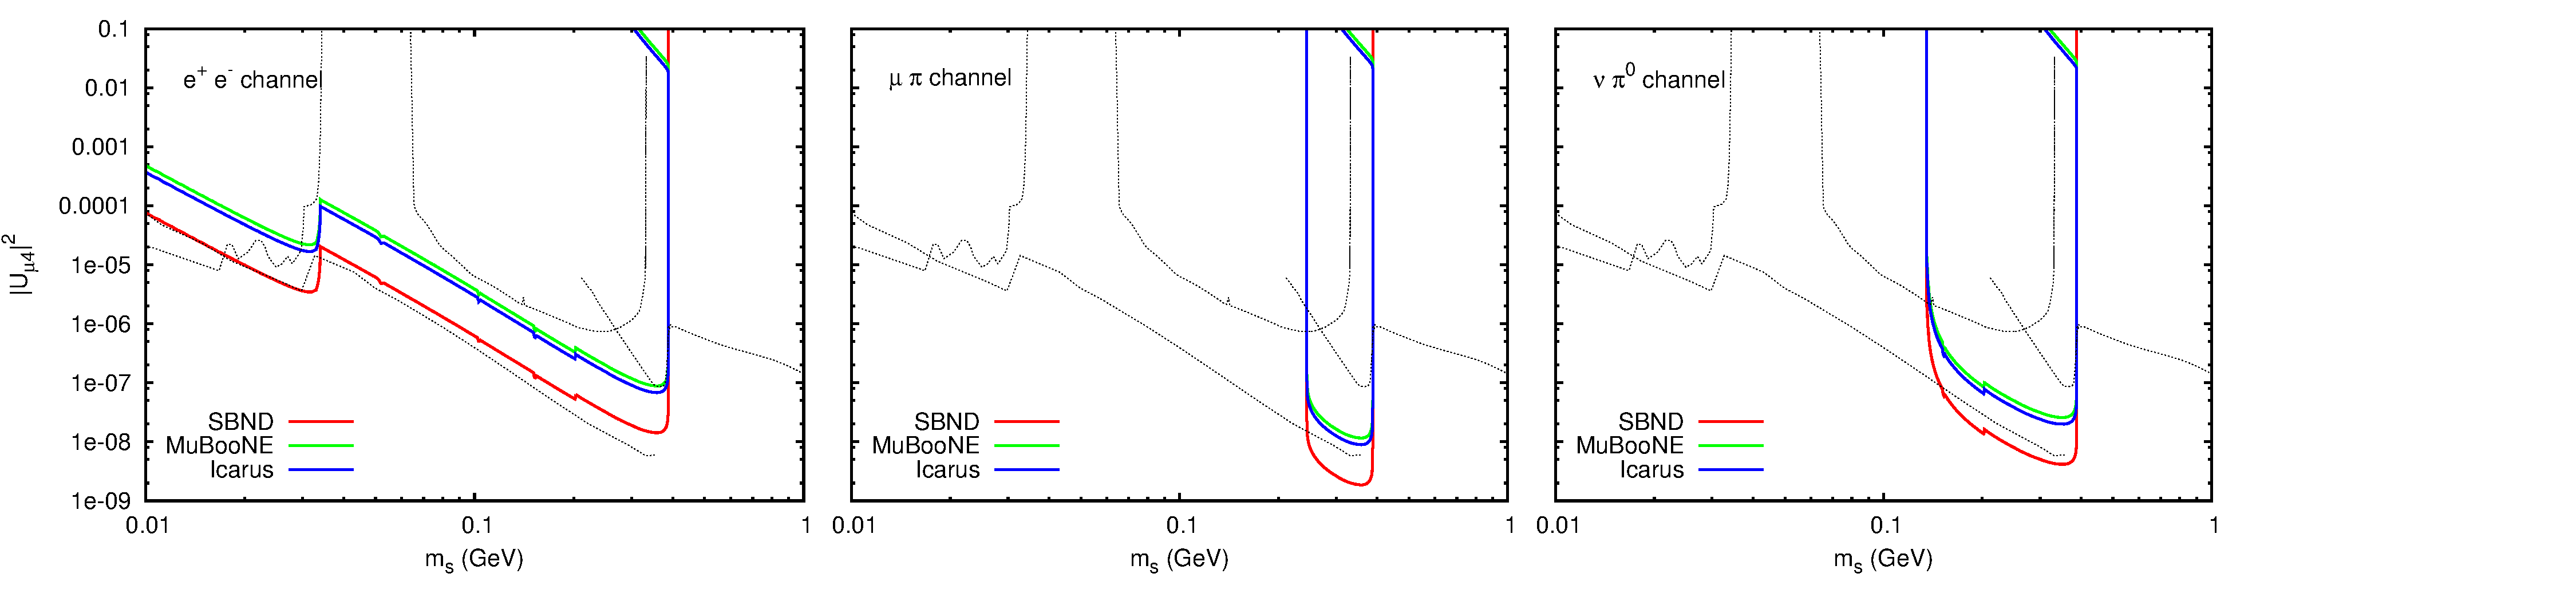
\includegraphics[width=1.0\textwidth,clip,trim=0 20 300 15]{figures/zerobg_um4_all_panels.pdf}
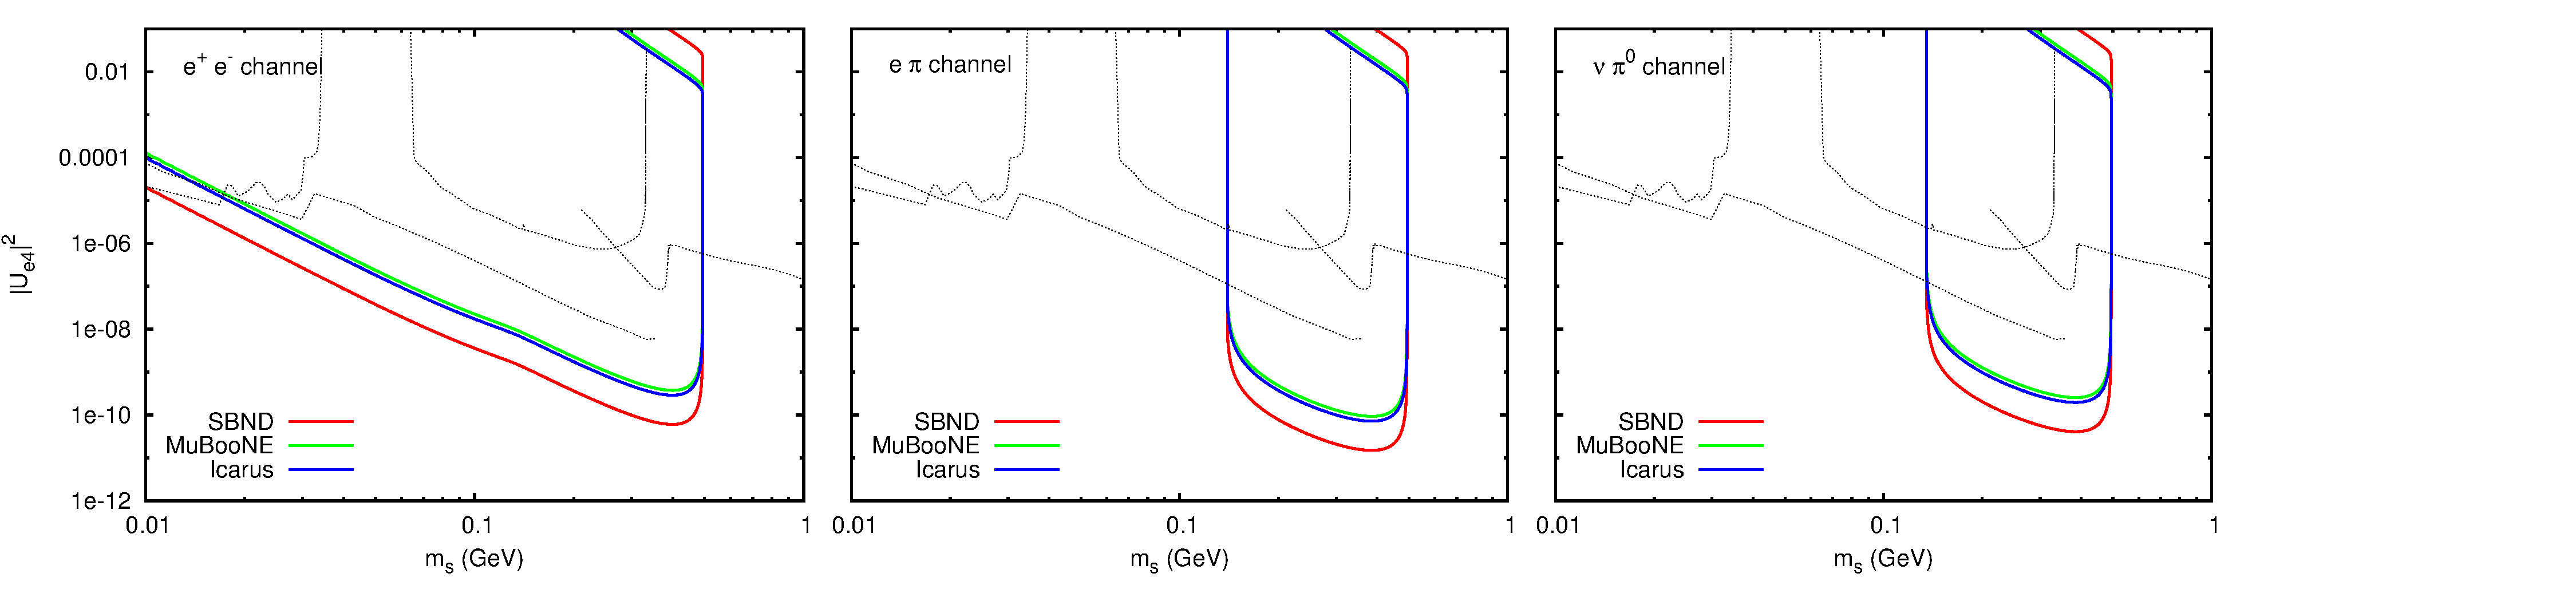
\includegraphics[width=1.0\textwidth,clip,trim=0 20 300 15]{figures/zerobg_ue4_all_panels.pdf}

\caption{\label{fig:no_cuts_no_bkg}The sensitivity contours based on the total number of events, without cuts and without backgrounds. In all panels, the mixing matrix elements not shown on the $y$-axis are zero.}

\end{figure}


\subsection{\label{sec:BMM}Beyond the Minimal Model}

\lorem\lorem

%In order to facilitate the search for new physics we provide results in terms
%of a total scaling $\Gamma$, of each decay channel of interest. We retain the
%functional dependance on sterile mass as in the minimal, bounding $\Gamma \vert
%U_{\alpha 4}\vert^2$. \\

%standard model weak processes with an active mixing scaling. Beyond this there
%are many extensions worth considering, if the sterile sector is charged under a
%new gauge symmetry, e.g $U(1)'$, then the total decay rate can be significantly
%modified. Additional new particle content that couples strongly with the sterile
%states can also drastically change the expected rate with respect to the minimal
%extension, as well as open up entirely new decay channels, such as the possible
%radioactive decay $\nu_N \rightarrow \nu_\alpha \gamma$, which can also be probed
%at the SBN and provides a window to searches for large sterile magnetic
%moments. In order to facilitate the search for new physics we provide results
%in terms of a total scaling $\Gamma$, of each decay channel of interest. We
%retain the functional dependence on sterile mass as in the minimal, bounding
%$\Gamma \vert U_{\alpha 4}\vert^2$. \\

%If there was an enhancement of $\alpha$ in a single channel, $\Gamma_c$, such
%that the total decay width becomes $\Gamma_\text{tot} =
%\Gamma_\text{oth}+\Gamma_c (1+\vert U_{\mu 4}\vert^2 \alpha)$, then previous
%experiments searching for heavy sterile decays would have had much more
%stringent bounds on $\vert U_{\mu 4} \vert^2$. We can estimate these enhanced
%bounds by comparing the probability to decay in a particular channel, with the
%probability associated with the published bounds, in particular we need to find
%the new value for the 90\% C.L bound, $\vert U_{\mu 4}\vert^2$, such that the
%probability to decay inside a detector of baseline L and length $\lambda$, with
%a total rate  $\Gamma_\text{tot} = \vert U_{\mu 4}\vert^2
%\left(\Gamma_\text{oth}^\prime+\Gamma_c^\prime (1+\alpha)\right)$, is equal to
%the probability to decay inside the same detector with total rate
%$\tilde{\Gamma}_\text{tot} = \vert U_{\mu 4}^*\vert^2(m_S)
%\left(\Gamma_\text{oth}^\prime+\Gamma_c^\prime\right)$, where $\vert U_{\mu
%4}^*\vert^2(m_S) $ indicates the published bound on that channel, for a sterile
%of mass $m_S$, and primed decay widths indicate the width with mixing removed
%to the front. Using the functional form of the probability in equation
%\ref{eq:prob}, and expanding to leading order in the assumed small parameter
%$\lambda/L$, there are two solutions to this corresponding to the two real
%branches of the Lambert-W function. The two solutions correspond physically to
%the cases where an increasing decay rate increases the number of observed
%events in a detector thus increasing the bound, $\mathcal{W}_0$, up until the
%decay rate becomes sufficiently large to ensure the majority of the events
%decay before reaching the detector, $\mathcal{W}_{-1}$. This places the 90\%
%C.L exclusion in a region \[	-\frac{\vert U_{\mu 4}^* \vert^2}{ \kappa
%\Gamma_\text{tot}^{*}} \mathcal{W}_{-1} \left[-\frac{\kappa
%\Gamma_\text{tot}^{*}}{1+\alpha} \exp\left(
%-\kappa(\Gamma_c^*+\Gamma_\text{oth}^*) \right)     \right]	\geq \vert
%U_{\mu 4} \vert^2 \geq \frac{\vert U_{\mu 4}^* \vert^2}{1+\alpha} \] where
%$\kappa = \frac{L}{\gamma \beta}$ and we have expanded $\mathcal{W}_0$ to
%leading order in $\vert U_{\mu 4}^*\vert^2$ for clarity to see it scales as
%expected with enhancement $(1+\alpha)$ , no such convenient expansion exists
%for  $\mathcal{W}_{-1}$.  

% 
%\begin{figure}[t]
%%
%\centering
%%
%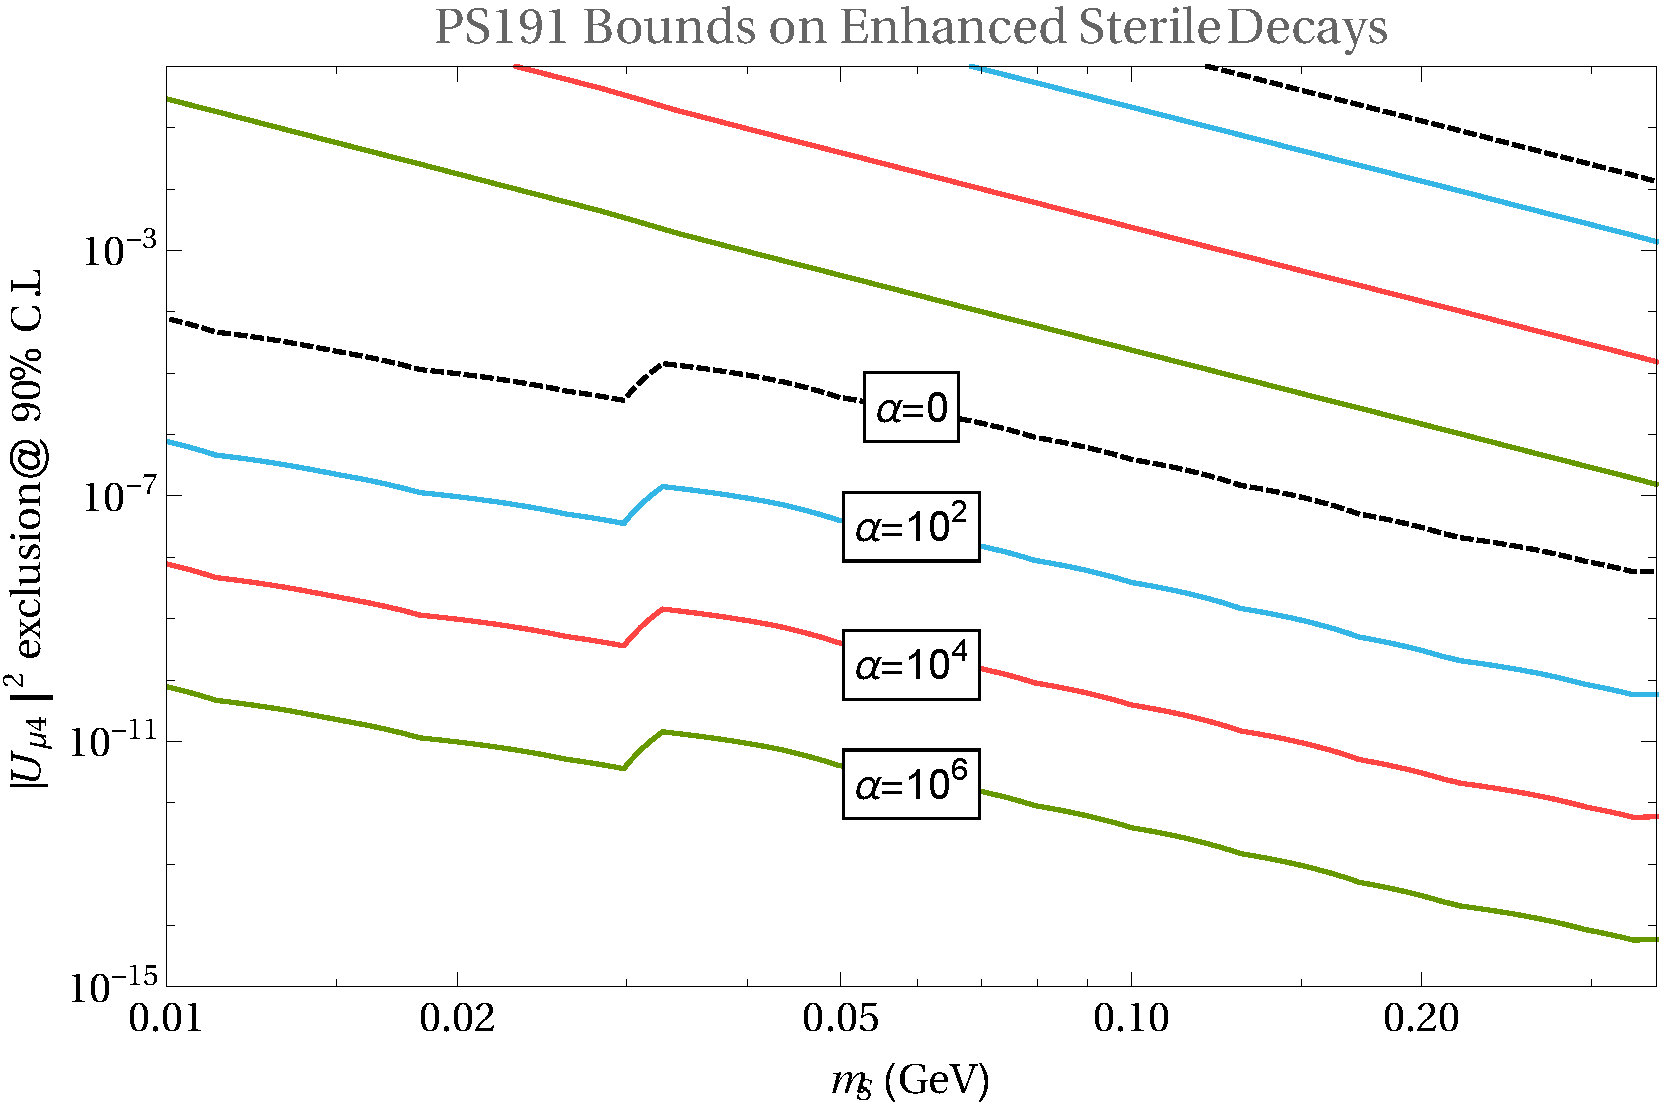
\includegraphics[width=0.49\textwidth]{figures/ps191_enhanced.pdf} 
%%
%\caption{\label{fig:ps191_enhance}The shifting of bounded region (excluded at
%90 \% C.L  between coloured line pairs) as the decay rate to a specific channel
%($\nu_N \rightarrow \nu_\mu e^+e^-$) is increased by an arbitrary scaling
%factor $\alpha$ at the PS-191 facility,$\alpha = 0$ corresponds to the minimal
%model bounds. A baseline of 128m, and mean energy of $\left< E_\nu \right>
%\approx 1 GeV$ was assumed.  , as well as the }
%%
%\end{figure}
%To investigate how the presence of backgrounds weaken these sensitivities, we
%have performed a rough estimate of the significance of the signal in various
%channels. In \reffig{fig:no_cuts_scaled_bkg}, we consider the quantity
%$S/\sqrt{\lambda B}$ and plot contours when the parameter is equal to $1$. At
%this point, the size of the new signal events from the heavy sterile decays are
%equal to the Poisson noise in the experiment under the approximation of no
%signal. The parameter $\lambda$ is used to scale the backgrounds, corresponding
%to a greater ability to suppresses these events.  We show two regions, the most
%conservative line corresponds to $\lambda=1$ with no additional background
%suppression beyond our estimates, whilst the more optimistic one corresponds to
%a further suppression by a factor of 1000. Our estimates are given by the
%largest numbers in \reftab{tab:rates} for each channel, that is assuming no
%analysis-based reduction in rates. As before, we do not take into account the
%signal efficiency in these plots (weight factors are set to $1$) this makes the
%unrealistic assumption that whatever has been done to reduce the backgrounds
%leaves the signal event rates unchanged. However, it provides an understanding of 
%the severity of the impact of the backgrounds for these searches.
%
%\newtext{PB}{Be careful: the contours aren't really the same thing as the
%shaded region, as they are computing different statistical quantities. But to
%make them into actual exclusion curves, we would have to minimize over the 2D
%space... which maybe we should do... but as we know it takes a bit of work.
%Also, the ee flux isn't quite right for a reason I forget at the moment.}
%
%
%\begin{figure}[t]
%\center
%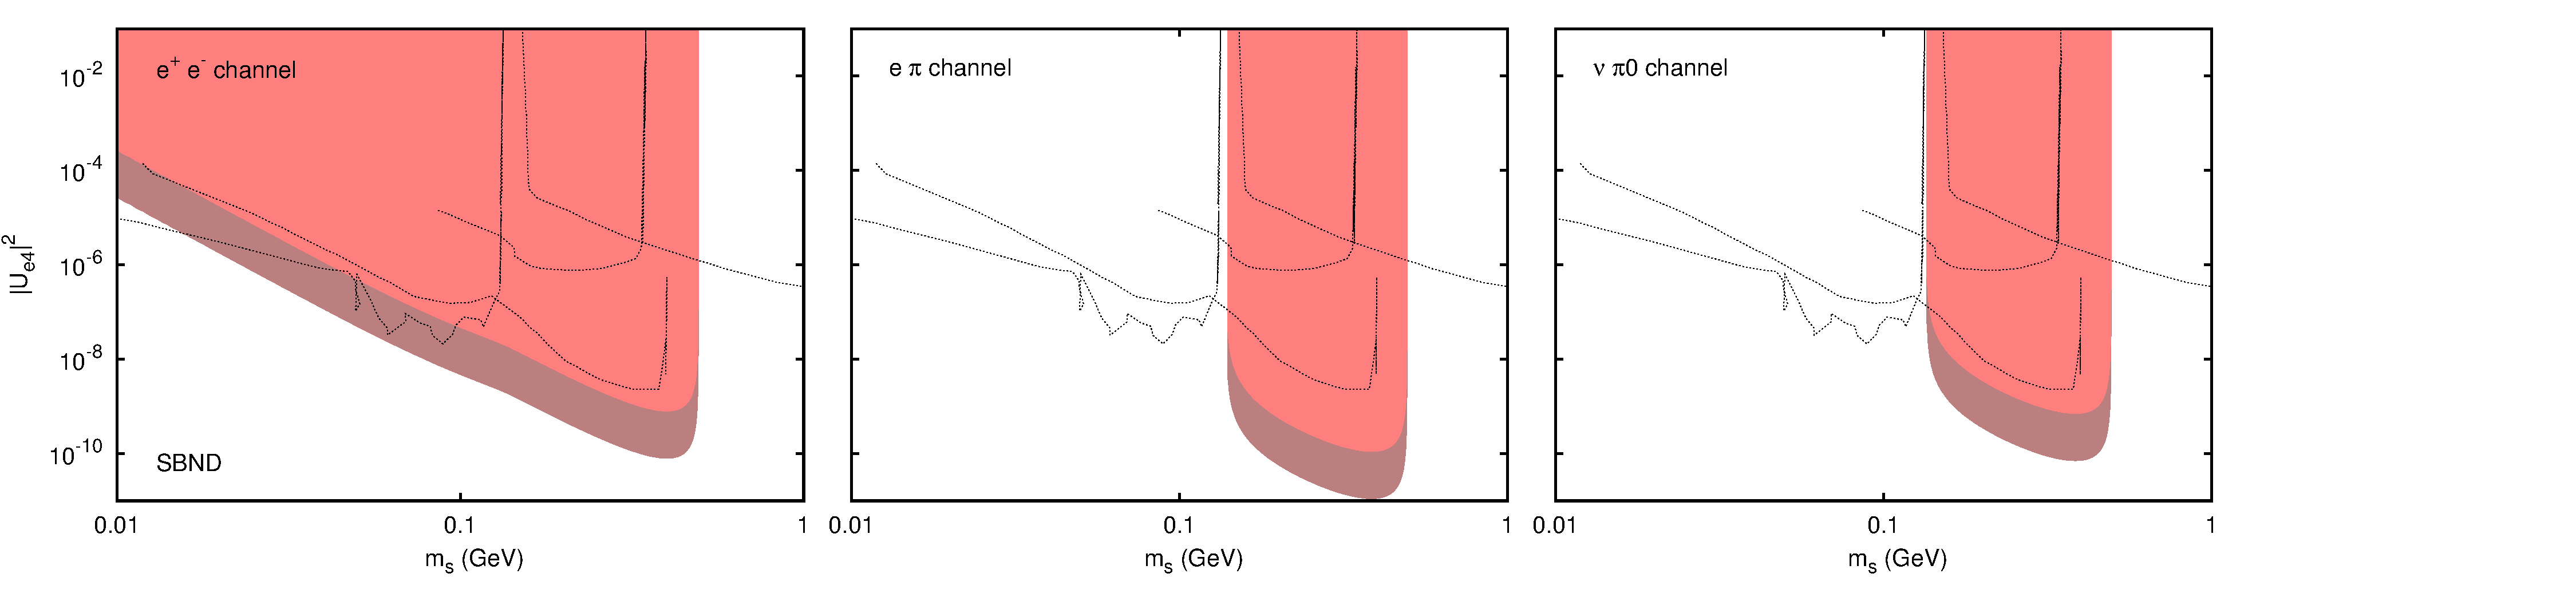
\includegraphics[width=1.0\textwidth,clip,trim=0 20 300 15]{figures/sbnd_all_panels_ue4.pdf}
%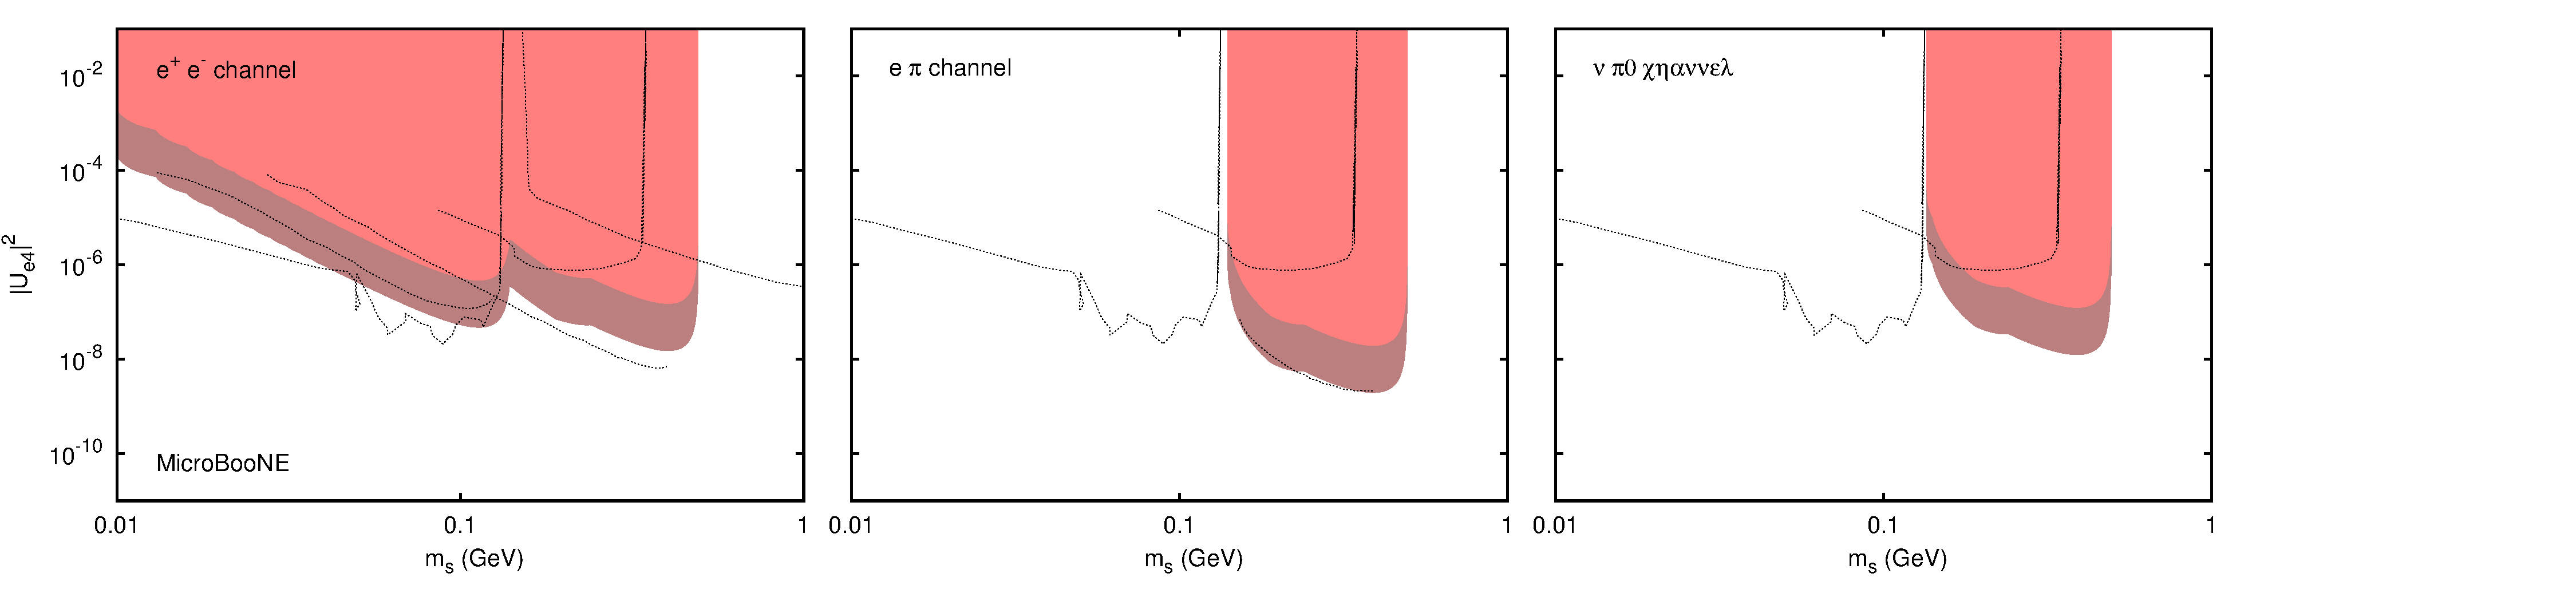
\includegraphics[width=1.0\textwidth,clip,trim=0 20 300 15]{figures/muboone_all_panels_ue4.pdf}
%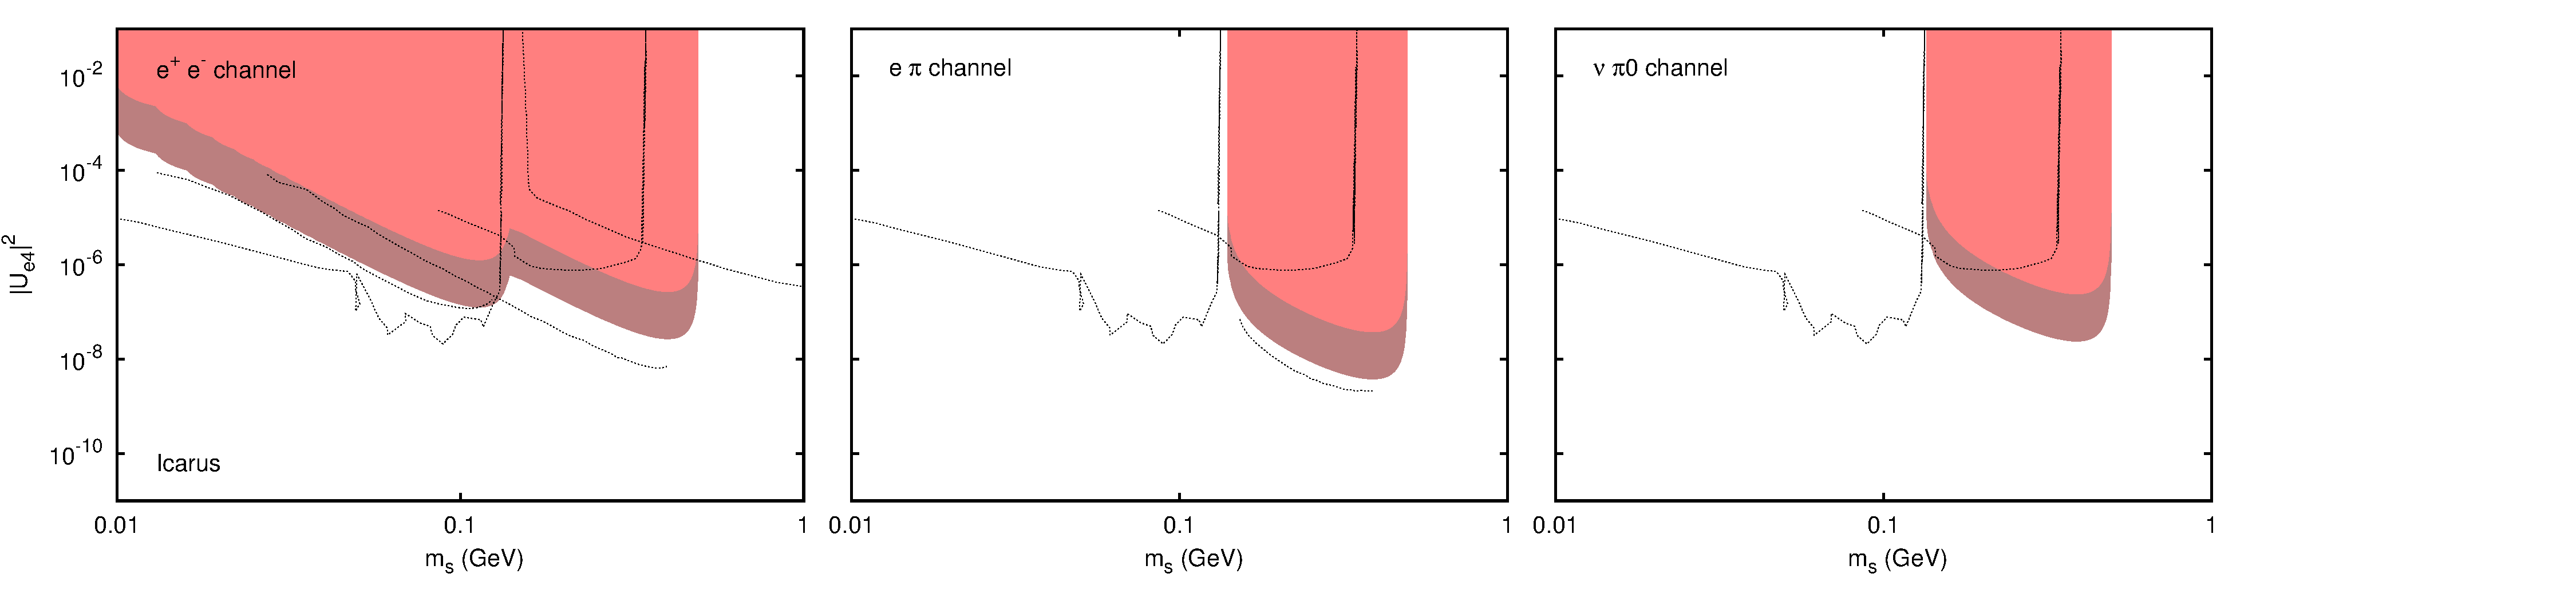
\includegraphics[width=1.0\textwidth,clip,trim=0 20 300 15]{figures/icarus_all_panels_ue4.pdf}
%
%\caption{\label{fig:no_cuts_scaled_bkg_ue4_only}The sensitivity contours based on the total
%	number of events, assuming only mixing with the electron neutrino ( $\vert U_{\mu 4}\vert^2=\vert U_{\tau 4}\vert^2=0$), without cuts but with varying degrees of background
%suppression. We overlay the 95\% exclusion regions for $U^2$ and $m_s$ from
%previous experimental work.}
%
%\end{figure}
%
%\begin{figure}[t]
%\center
%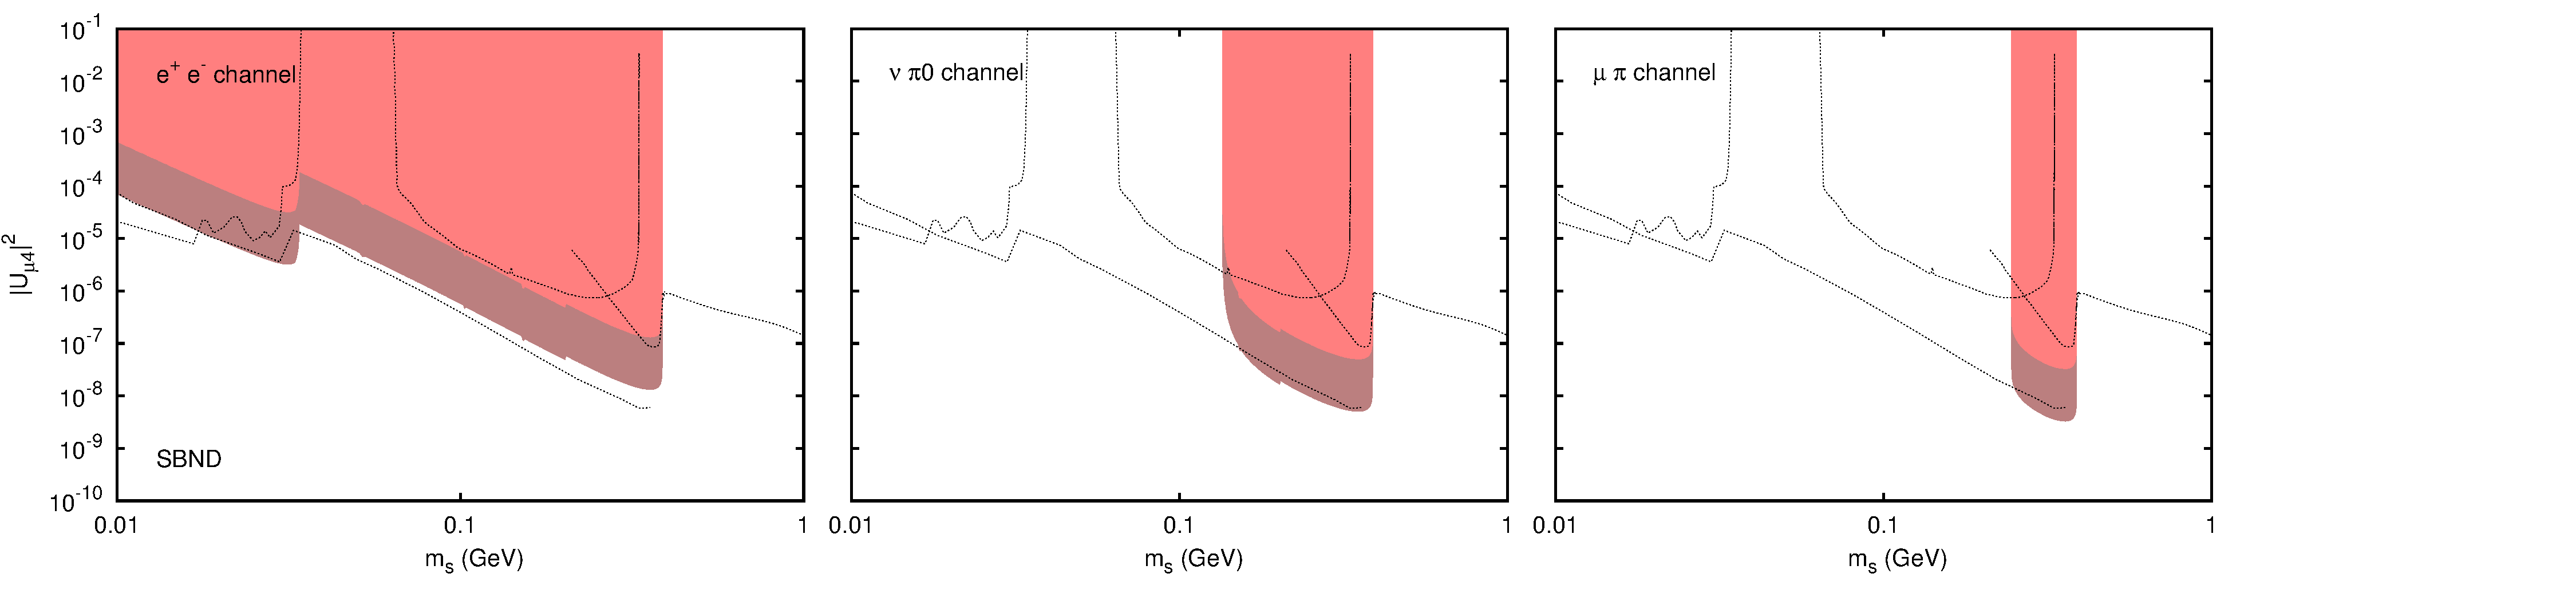
\includegraphics[width=1.0\textwidth,clip,trim=0 20 300 15]{figures/sbnd_all_panels_um4.pdf}
%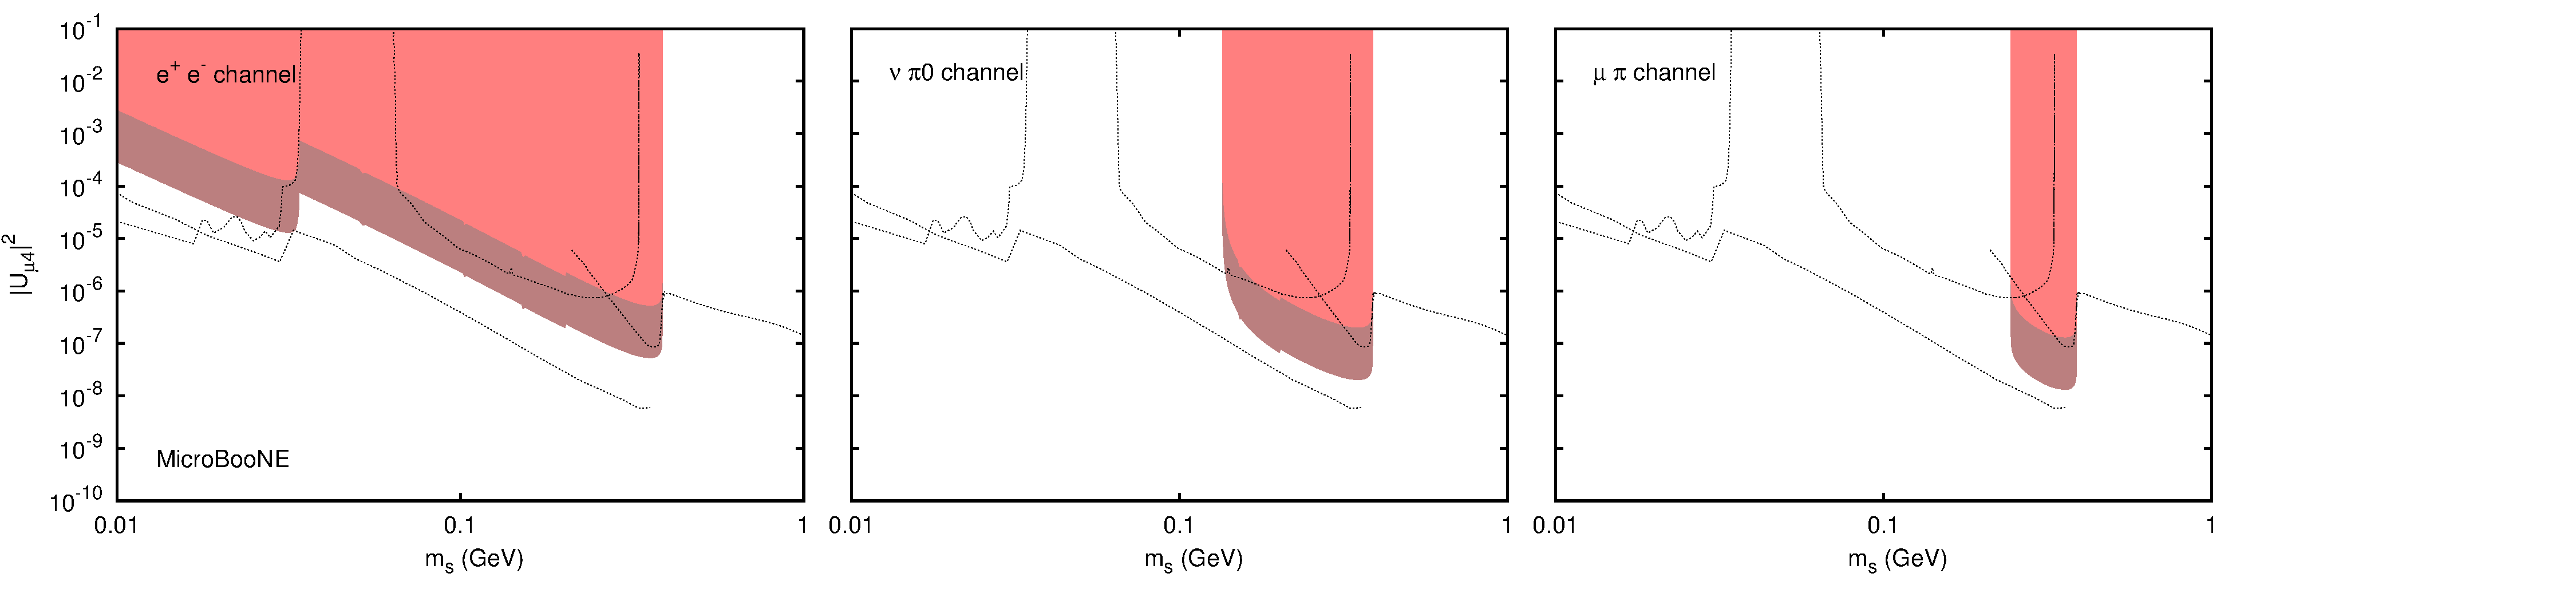
\includegraphics[width=1.0\textwidth,clip,trim=0 20 300 15]{figures/muboone_all_panels_um4.pdf}
%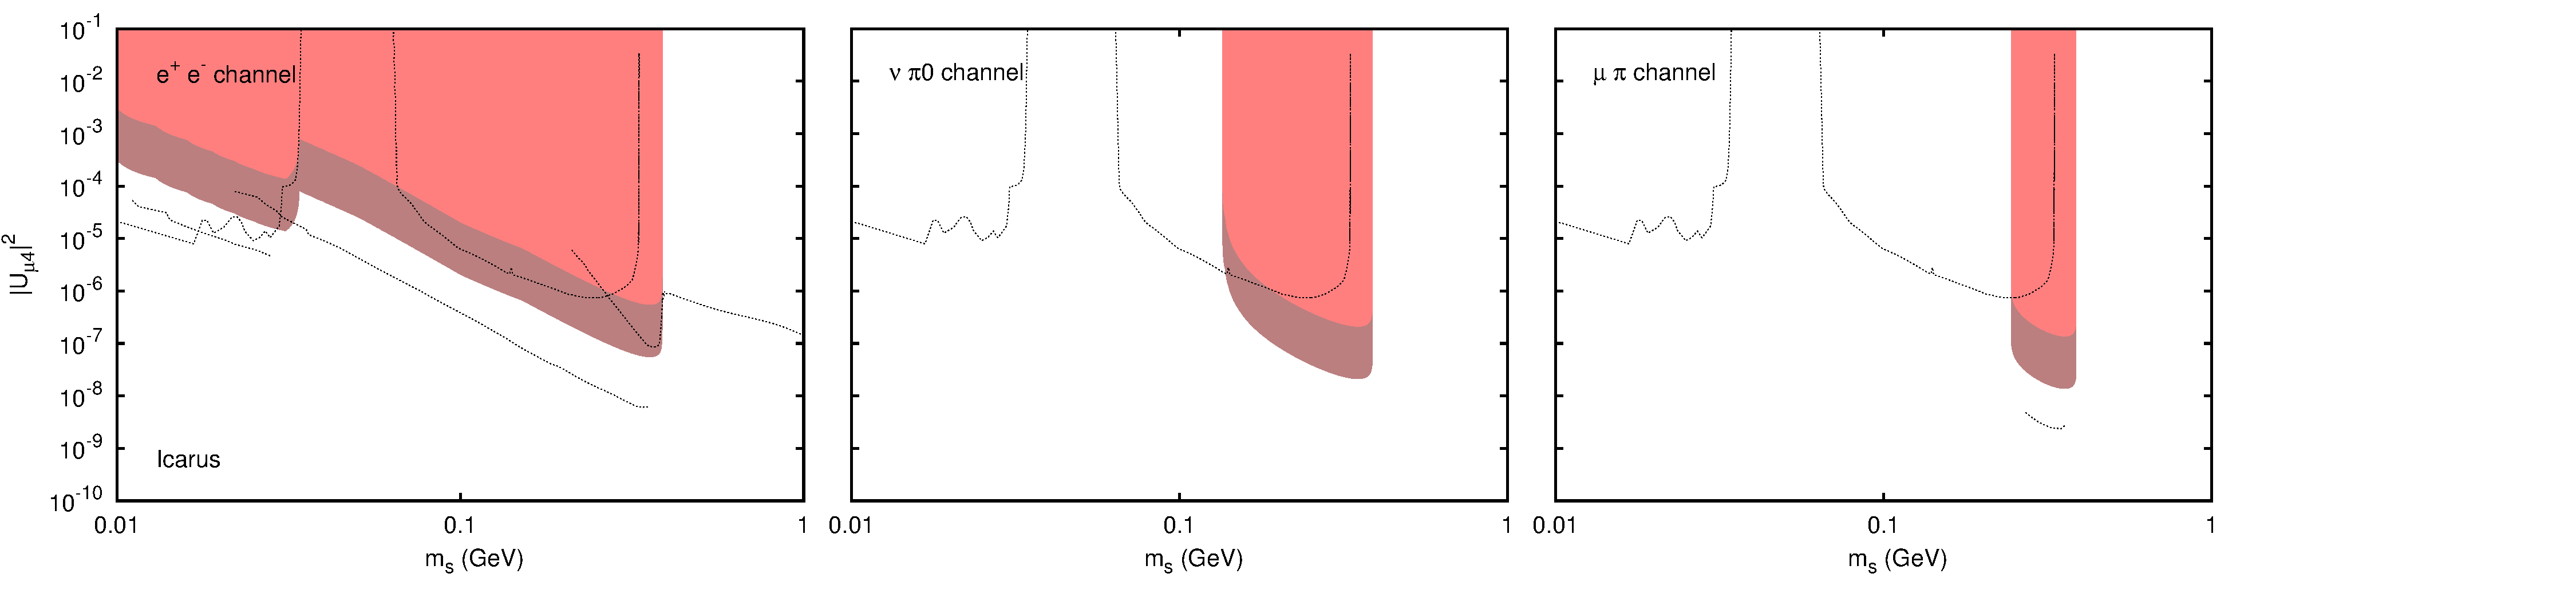
\includegraphics[width=1.0\textwidth,clip,trim=0 20 300 15]{figures/icarus_all_panels_um4.pdf}
%
%\caption{\label{fig:no_cuts_scaled_bkg_um4_only}The sensitivity contours based on the total
%number of events, assuming only mixing with the muon neutrino ( $\vert U_{e 4}\vert^2=\vert U_{\tau 4}\vert^2=0$), without cuts but with varying degrees of background
%suppression. We overlay the 95\% exclusion regions for $U^2$ and $m_s$ from
%previous experimental work.}
%
%\end{figure}
%

\section{Background Analysis\label{sec:bg}}
In this section we will discuss the predominant beam-releated backgrounds to detection of a decaying sterile neutrino. Historically, such decay in flight experiments utilised low mass detectors to minimize neutrino induced CC and NC scattering events. We will argue, however, that the distinct kinematics of a decay compared to that of a beam induced scattering background event, in conjunction with the angular and energy resolution of LAr detectors, allows the three SBN facilities to work in an near backgroundless environment for many of the discussed channels.

In order to show this we have performed a full Monte-Carlo analysis of the expected backgrounds using the neutrino event generator GENIE. This provides us with generator level information about the kinematics of the beam-driven backgrounds, with rates normalised off expected NC and CC inclusive values as published in the SBN proposal. Energy and angular smearing is then implemented to allow for approximate estimates of the effects of detector performance to the level necessary for this analysis, without the need for a full GEANT detector simulation. Energies are smeared according to a Gaussian distribution around their true MC energies, with a relative variance $\sigma_E/E = \xi/ \sqrt(E) $, where $\xi$ is a detector dependant resolution. For this study we take the energy resolution for EM showers, muons and protons to be 15\%, 6\% and a conservative 15\% respectively. We take the angular resolution of LAr to be $1^{\circ}$. 

Of utmost importance in all studied channels to distinguishing signal and background is the identification of a scattering vertex. Any hadronic activity localized at the beginning of the lepton track is a smoking gun signal for beam related scattering from deep-inelastic or quasi-elastic scattering. Therefore any event containing one or more reconstructed protons or additional hadrons is rejected outright. For counting this proton multiplicity we assume an detection threshold of 21 MeV on proton kinetic energy in liquid Argon, after smearing. Background events that contain less than this and events that do not contain any protons, such as events originating from coherent pion production, remain a viable background and further rejection must come from the kinematics of the final state particles only. The properties of these backgrounds will be what most strongly motivates our cuts. We will discuss the details of the modelling that we have performed in a channel-by-channel basis. 

\begin{figure}[h]
\center
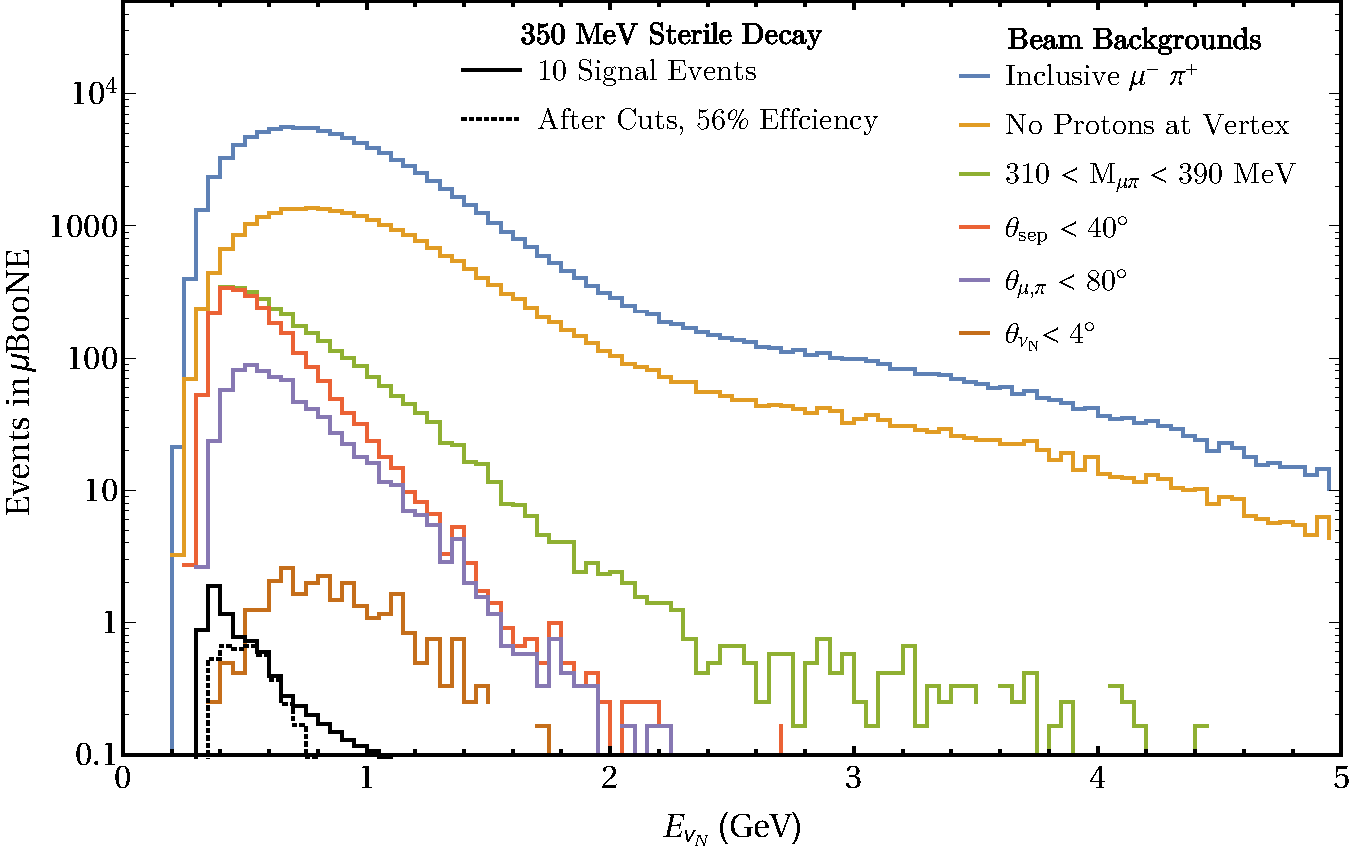
\includegraphics[width=0.6\textwidth,clip,trim=0 0 0 0]{figures/mu_pi_cutflow.pdf}
\caption{\label{fig:mu_pi_cutflow} Reconstructed sterile energy spectra for CC$\nu_\mu$ backgrounds in comparason to a 350 MeV decaying sterile at $\mu$BooNE, normalised to 10 signal events. Total expected background of 98,013 events is reduced to $\approx$ 27 by successive kinematic cuts utilising expected differences between decay and scattering behaviour. }

\end{figure}
\subsection{$\nu_N \rightarrow \mu^\pm \pi^\mp$ }

Pions produced inside the SBN LAr detectors will quickly decay into muons,
which either escape the detector, or if low enough energy, subsequently decay into Michel electrons and the entire track is contained inside the active volume. We can expect this chain of decays to be well reconstructed in liquid argon if the
pion and muon are contained. As there are no additional active neutrinos present this channel to take away missing energy the exact kinematics of the parent sterile can be reconstructed and allows for strong background rejection. 

The dominant backgrounds to the sterile decays we are interested in will be genuine $\pi$-lepton production associated with
the neutrino beam. So-called CC1$\pi^+$ events are defined as the associated production of a charged pion from the standard CC process which produces a lepton. This can happen by resonant production, where a nucleon is excited into
an unstable state, for example into a $\Delta$, and the following decay
produces a nucleon and a pion. Such decays are characterized by a a relatively
isotropic spectrum due to the relatively mild boost of the resonant state
\cite{Rein:1982pf}. 

Another contribution to the cross-section is from coherent scattering, where
the neutrino scatters from the whole nucleus. These interactions tend to produce more forward decay products and will be
another significant source of backgrounds. Cross-sections for these processes have been studied in MiniBooNE \cite{Wascko:2006tx} and \minerva\
\cite{Eberly:2014mra} and cross-sections appear to agree with Monte Carlo calculations based on the Rein-Sehgal model \cite{Rein:2006di, Rein:1982pf}.
Such a low $Q^2$ process tends to favour daughter pions and muons that are forward going, kinematically very similar to decays in flight, as well as no observable nuclear activity.\\ 

The strongest desctriminator between background and signal is the reconstructed angle of parent sterile, $\theta_N$. Any $\mu^-$-$\pi^+$ pairs from CC scattering events tend to reconstruct to a broad contonous dropping spectrum as the event is not a true two-body decay, while signal events are highly forward-going with $\approx 95$\% below $4^\circ$ relative to the beamline. Additionally, information of the reconstructed invariant mass of the lepton pion pair, $M_{l^\pm \pi^\mp}^2=m_l^2+m_{p^\pm}^2+ 2(E_l E_\pi - |P_l||P_\pi|\cos\theta_\text{sep})$, will sum to that of the the parent sterile (within detector resolution), where as the background is expected form a broad spectra spanning the energies of incoming neutrino. We therefore implement an additional cut on any events whose invariant mass is outside an 80 MeV window surrounding the parent sterile mass. The effect of these cuts, alongside that of the stringent requirement of no visible vertex, reduces the potential background of $\mu^- \pi^+$ events from 1,153,090 in SBND to approximately 323 events. Figure (\ref{fig:mu_pi_cutflow}) shows the background rejection capability of LAr as each additional cut is implemented.

\subsection{$\nu_N \rightarrow e^\pm \pi^\mp$ }
If there is a non-zero $U_{e4}$ then the decay to electron and charged pion opens up when $m_\pi +m_e \leq m_N \leq m_K$. The expected numbers of $e \pi$ events in the SBN detectors is significantly smaller than that of the $\mu \pi$ channel, as the fraction of intrinsic $\nu_e$ in the BNB beam is of
$\mathcal{O}(1\%)$ level in comparason to $\nu_\mu$. However, there will also be additional backgrounds to the
$e \pi$ channel originating from the dominant $\nu_\mu$ beam. CC $\nu_\mu$ events which contain an additional photon $(\mu+\gamma)$, or 1 reconstructed photon from a $\pi^0$ decay, have the potential to be be mis-identified as an $(\pi
e)$ event, provided the muon has a sufficiently short track length, $<$ 0.5 m, in order to mimic a $\pi^-$. Additionally the photon must be mis-identified as an electron, with an efficiency of 94\%, and furthermore, must convert to an $e^+e^-$ pair close enough to the interaction vertex as so there is no visible gap. Thus we accept 6\% of all CC $\mu+\gamma$ events whose photon converts within 3cm, and whose muon track length is less than 0.5m. Combined with the rejection of events with any vertex activity, this reduces the number of background events to below that expected from intrinsic CC $\nu_e$ pion production. As energy resolution for EM showers is lower than muons, the invariant mass cut is less powerful requiring all events have an invariant mass below 500 MeV. We also cut on reconstructed sterile angle, and seperation between  $e^-$ and $\pi^+$ identically to $\mu^- \pi^+$ channel above. The $e^- \pi^+$ channel is one of the cleanest channel under consideration, with 9223 events in SBND reducing to 22 expected events post cuts, and with $\mu$BooNE and ICARUS expecting $\mathcal{O}(1)$ events from beam driven backgrounds.


\subsection{$\nu_N \rightarrow \nu_\alpha e^+ e^-$ }

A sufficiently boosted, and thus overlapping, $e^+e^-$ pair is topoligically indistinguishable from a converted photon in a LAr detector. Topology is not the only means of distinguising photons and electrons in liquid argon, however, they also have a non-topological method for distinguishing electrons from photons via the rate of energy loss $dE/dx$, naively one would expect a photon which pair produces to loose energy at a rate twice that of a single electron. For a sufficicently collimated $e^+e^-$ pair, however, this rate of energy loss would also match up with that of a pair-converted photon, meaning separation is near impossible. Thus we split this channel into two sub categeories, when the $e^+e^-$ is overlapping and photon-like, defined to be all events whose angular seperation is $\leq 3^\circ$\cite{Spitz:2011wba} and all remaining seperable two track events. The opening angle between the $e^+e^-$ in a photon pair production scales roughly as $\approx m_e/E_\gamma$, with $3^\circ$ corresponding to 100 MeV and used as a lower bound on energy. The majority of such overlapping events originate from low mass parent steriles, $\leq 50$ MeV\\ 

Any standard process producing a lone stray photon is thus a possible source of backgrounds for the photon-like $e^+e^-$ channel. The predominant source of this in all three SBN detectors is the decay of a neutral pion in which a single photon is not resolved or escapes the fiducial volume. This background, however, is relatively isotropic in distribution and of lower energy that the signal, in stark contrast to the very forward, and energetic signal, as can be seen in Figure \ref{fig:gamma_dist} below. Thus we apply a cut on visible photon energy, $E_\gamma \geq 300 $ MeV and angle of the observed photon to the beamline, $\theta_\gamma \leq 5^\circ$. In conjunction with the requirement that no vertex activity is recorded, this reduced the number of expeceted events from 42,580 to 76 events in SBND, while retaining a signal efficiency of 93\%.

For the opposite scenario, in which both daughter electrons have a well defined, and large, separation and thus can cleanly be identified as two distinct single electron showers, the expected background sources are different. There are no significant` processes that produce high energy, distinguishable $e^+e^-$ pairs at the SBNs.  Instead the majority of the backgrounds are due to misidentifying photons, which are abundant, as electrons. A principle background is CC $\nu_e N \rightarrow e^- N^\prime \gamma$ interactions in which the electron is accompanied by a photon which is mis-identified as an electron. This single photon can be emmitted directly in the scattering, or can be the result of a $\pi^0$ decay in which one photon is not detected. Additionally the common NC  process $\nu_\mu N \rightarrow \nu_\mu N \pi^0$, and subsequent $\pi^0$ decay in which both of the underlying photons are mis-identified as electrons. As both of these backgrounds require the photons to mimic electrons originating from a single decay vertex, we also require that all photons pair convert within 3cm of the start of the electron track in the case of CC $\nu_e$ backgrounds, or both photons convert within 3cm of each other in the case of NC $\pi^0$ backgrounds. Further more, each event passing the above cuts is rejected with a 94\% efficiency using measurements of the rate of energy loss, $dE\/dx$. All remaining events are kept as backgrounds. As an active neutrino is involved removing an unknown amount of energy, the energy and angle of the parent sterile cannot be directly reconstructed and the invariant mass of the $e^+ e^-$ no longer can be used to discriminate from background. Alongside the insistence of no reconstructed vertex, to further recject backgrounds we apply a cut on angle of speration between the distict $e^-e^-$ tracks of $\theta_\text{sep}\leq 40 ^\circ$ and total energy, $E_{e^+}+E_{e^-} \geq 100$ MeV.This reduces the number of expected backgrounds from 173 events to 5 events in SBND. 

\begin{figure}[h]
\center
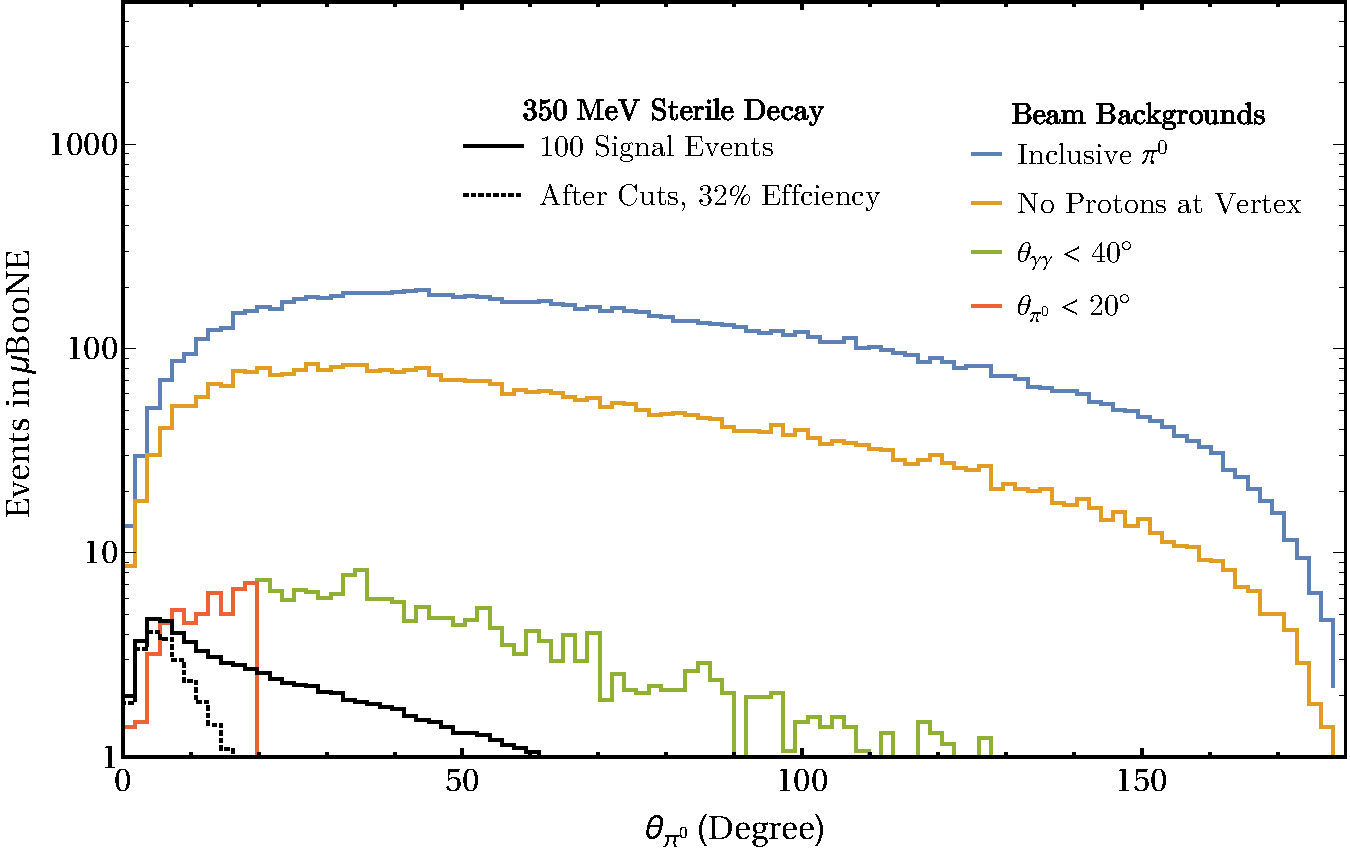
\includegraphics[width=0.6\textwidth,clip,trim=0 0 0 0]{figures/nu_pi0_cutflow.pdf}
\caption{\label{fig:nu_pi0_cutflow} Reconstructed $\pi^0$ angular spectra with respect to the beamline for NC$\nu_\mu$ backgrounds in comparason to a 350 MeV decaying sterile $\nu_N \rightarrow \nu_\alpha \pi^0$ at $\mu$BooNE, normalised to 100 signal events. Total expected background of 10,813 events is reduced to $\approx$ 51 by utilising forwardness of pion produced in decays, alonside the requirement of no hadronic activity. }

\end{figure}

\subsection{$\nu_N \rightarrow \pi^0 \nu_\alpha$}
Although a sub-dominant decay mode when steriles mix with electrons alone, when one considers non-zero $\vert U_{\mu4}\vert^2$ the branching ratio of $\nu_s \rightarrow \nu_\mu \pi^0$ becomes dominant for a mass window $\approx 140 \rightarrow 240$ MeV. There is no known experimental publication of $\nu_N \rightarrow \nu_\alpha \pi^0$ in the literature, mainly due to the large expected backgrounds. Single neutral pions are produced in great numbers at the three SBN facilities, so the lack of any nuclear recoil is crucial in eliminating the incoherent neutral pion production background. The NC coherent pion production, however, does not contain any nuclear tracks and so will be an irreducible background for this channel, up to spectral kinematics. As the $\pi^0$ itself is not visible, we focus on the reconstructed pion energy and angle, infered from measuring the resultant photons energy and angle, smeared as usual to model detector effects. Only events in which both photons convert inside the fiducial volume are accepted. Figure (\ref{fig:nu_pi0Pcutflow}) shows the angular spectrum of produced pions for signal and background before and after kinematic cuts. SBND expects 127,211 $\pi^0$ events, of which $\approx 602$ survive all cuts with a signal efficiceny of 32\% for an example 350 MeV sterile. \\ 

To summerise, we collect the total numbers of beam-induced background events expected at the three SBN below in Table (\ref{tab:Rates}), both before and after we apply all visible vertex and kinemaic cuts as described above. One can see that LAr provides an impressive level of background rejection, with \muboone and ICARUS being close to backgroundless in many channels, and SBND expecting only $\mathcal{O}(100)$ events in all channels.




\begin{table}[t]
\centering
\begin{tabular}{ l | l | l| l | l}
	Signal Channel & Main Backgrounds & Events @ SBND & \muboone\ & ICARUS \\
\hline\hline
\multirow{2}{*}{$\mu^\pm \pi^\mp$} & CC: $\nu_\mu  \rightarrow \mu \pi  $ & 1,530,900  & 98,013 & 164,716\\
													 & w/ Cuts &323 & 27 & 46 \\ \hline
\multirow{2}{*}{$ e^\pm \pi^\mp$} & CC: $\nu_e  \rightarrow e \pi  $ & 9,228  & 784 & 1,317\\
													 & w/ Cuts &22 & 2 & 3 \\ \hline
\multirow{2}{*}{$ \nu_\alpha \pi^0$} & NC: $\nu_\mu  \rightarrow \nu_\mu \pi^0 $ &  127,217 & 10,813 & 18,172\\
													 & w/ Cuts &603 & 51 & 86 \\ \hline
 \multirow{2}{*}{$ e^+e^- \text{ (Seperate)} $} & CC: $\nu_e  \rightarrow e \gamma  $ &  172 & 14 & 24\\
													 & w/ Cuts &3.5 & 0.3 & 0.5\\ \hline
  \multirow{2}{*}{$ e^+ e^- \text{ (Photon-like)}$} & NC: $\nu_\mu  \rightarrow \nu_\mu \gamma $ &  42,580 & 3,620 & 6,082\\
													 & w/ Cuts &176 & 46 & 110 \\ 
 \hline \hline

\end{tabular}
\caption{\label{tab:Rates} A summary of the main sources of backgrounds for each channel studied, before and after spectral and particle ID cuts are applied. }
\end{table}



\subsection{Non-Beam related backgrounds}
Cosmogenic backgrounds are expected to be significantly smaller in comparison to beam related backgrounds. In the case of cosmic muons, Icarus expects to see approximately $2.5 \times 10^{6}$ cosmic events in the 211 second beam spill,
and are reduced to approximately 5 events expected after utilizing the spill
structure, scintillation light patterns and cuts on $\frac{d E}{d x}$
\cite{Antonello:2015lea}. Similarly for cosmic backgrounds to electron (photon)
like signals 170 (146), 136 (88) and 498 (154) are expected at SBND, \muboone\
and Icarus respectively, however, they are predominately in the low energy
bins, $< 0.5$ GeV. Alongside this impressive cosmic rejection, our signal
events are focused heavily along the beamline, hence we do not expect cosmics
to be a major source of background to any channel are are not included in this
analysis. Total flux uncertainties have little effect on the resultant
sensitivities as shifts affects both signal and beam driven background equally.
Cross-sectional uncertainties, however, have the potential to modify all beam
related backgrounds while leaving the decay in flight signal unchanged and thus
are an unavoidable source of uncertainty.




\section{\label{sec:baselineinterplay}Baseline dependence at the SBN complex}
The combination of three detectors, all operating with the same technology in
the same neutrino beam allows for distinctive signatures of new physics. By
studying the dependence of the signal on baseline and detector mass, we could
hope to further constrain the model underlying explanations of any observed
excess.  

In this section we will discuss two ways to constrain new physics if an excess
of events is observed. First, we focus on the ways that event numbers scale
between the detectors and in which scenarios we could identify the origins of
an excess of events. Secondly, we discuss the role of timing on model selection.
Timing delays between excesses would be strong evidence for heavy particles 
propagating between source and detector, and we explore how the study of timing
effects could be used to bound the mass of the particle in a model independent 
fashion.

\subsection{Scaling behaviour of event rates}
%
%\begin{figure}[t]
%%
%\centering
%%
%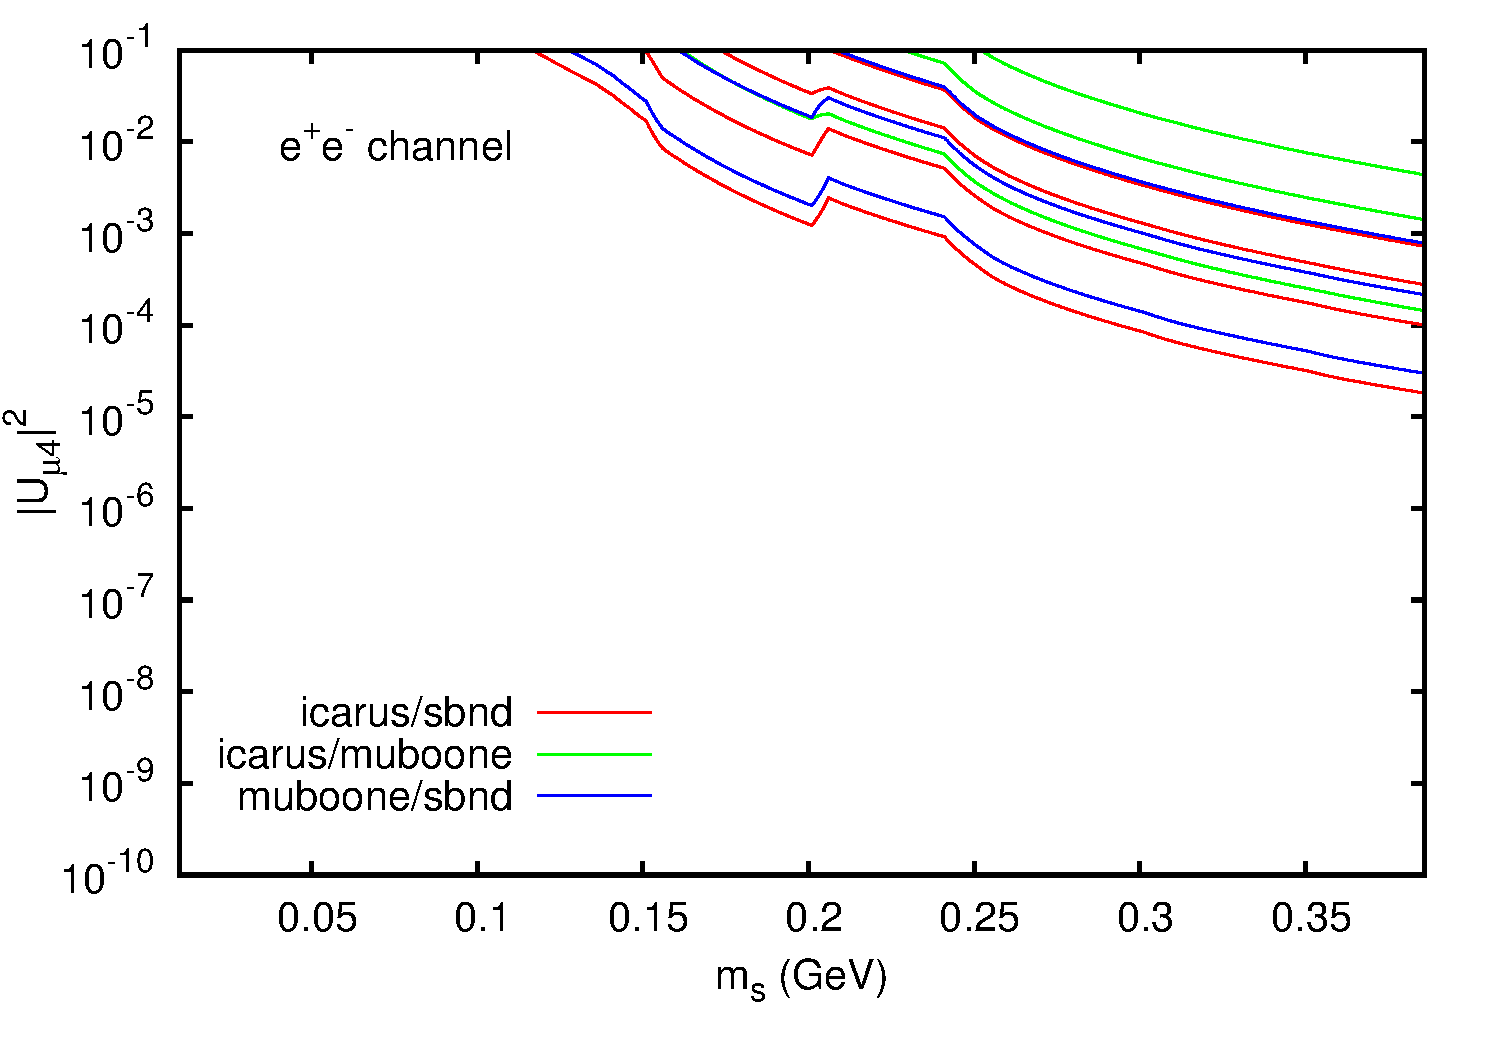
\includegraphics[width=0.49\textwidth,clip,trim=0 20 35 10]{figures/baselineratios_ee_um4.pdf} 
%%
%\caption{\label{fig:baselineratios} The ratio of event numbers for the $e^+e^-$
%decay channel between the three detectors as a function of mass and mixing in
%the minimal extension to the SM.  All the regions towards the lower-left
%predict a ratio of $1$ between the observed excesses, and the contours show the
%lines for excess-ratios of less than 1, 0.75, 0.5 and 0.25. The ratios have been scaled
%to account for the dependence of the flux on baseline, and the difference comes
%purely from the attenuation of the beam due to decays in transit between source
%and detector. }
%%
%\end{figure}

An excess of events at a detector often has multiple competing explanations.
However, in most physical scenarios the scaling behaviour of the predicted
number of events will differ. For example, any source of excess events which is
induced by the neutrino beam should inherit a $L^{-2}$ dependence on baseline
distance from the dispersion of the neutrino flux. Between three detectors,
this would generate a distinctive relative enhancement of the signal at SBND
and relative suppression of the signal at ICARUS compared to a fixed nominal
excess at \muboone. This is in contrast to, for example, an excess of
misidentified cosmogenic events which would have no baseline dependence.

New physics may cause a signficant dependence on baseline. One of the much
discussed ways to explain an excess of events at a short baseline neutrino
experiment is through sterile neutrino oscillations. The rates predicted at
three different detectors depend crucially on the respective distances from
source to detector according to the oscillation prbobability. In the scenarios
discussed in this paper, we also see baseline dependence coming from
\refeq{eq:prob}, albeit in a very different form. For most of the parameter
space, we would predict no significant baseline dependence on the event rates
at the three detectors, once the $1/L^2$ dependence of the flux is removed;
however, for large decay rates we see a baseline dependent effect. This is
shown in \reffig{fig:baselineratios}, where the event numbers for $e^-e^-$
decay are shown as ratios between the three detectors. These have been scaled
to remove the baseline dependence of the flux.  The four lines for each
detector show the 100\%, 75\%, 50\% and 25\% contours (where the further
detector sees fewer events). Such decay rates are forbidden in the minimal
extension of the SM incorporating MeV scale sterile neutrinos
\newtext{PB}{True?}. In a non-minimal model, it remains possible that decays
with decay lengths of the order $100$~m could exist, leading to a very 
significant depletion of events at the further detectors.

We show in \reffig{fig:baselineratios} a plot highlighting the contrasting
behaviour between these alternative explanations for an excess seen at the SBN
complex. In these plots we assume a fixed $100$ events at \muboone\ and observe
the distribution of events at the other sites for different models of new
physics.

\subsection{\label{sec:timing_physics}Timing for model discrimination}

A unique feature of the SBN complex is its combination of three detectors
situated at distinct baselines. One opportunity that this suggests is the
observation of time delayed signals between the sites. As particles with finite
rest mass, the heavy neutral leptons will propagate at subluminal speeds and
for larger masses can produce observable timing delays. If an excess of events
is observed with a clear timing delay between SBND and Icarus, this would be
very difficult to explain using an oscillatory sterile, neutrino induced
beam-correlated signal or other non-beam background and would be a clear
indication of a heavy propagating degree of freedom. 

We can estimate the impact of this information on the model discrimination
given an knowledge of the precision in timing measurements of the sterile
neutrinos. Elementary special relativity tells us that for an arrival time delay (behind a luminal particle) over a distance $L$ denoted by $\Delta T$, the mass of a sterile neutrino with an energy $E$ can be reconstructed as 
%
%\[    \Delta T = \frac{L}{c}\left(\frac{E}{\sqrt{E^2-m_\text{s}^2}} - 1\right). \]
%
\[ m_\text{s} = E\sqrt{1-\frac{1}{\left(1+\frac{c\Delta T}{L}\right)^2}}. \]

To determine the prospects for measuring $m_\text{s}$ using this information we
have generated Monte Carlo event data tagging each event by an arrival time.
We account for a systematic uncertainty associated with the time measurement as
well as the energy reconstruction. From \refref{WHERE}, we take a Gaussian
smeared energy resolution of around $\sigma_E \approx ??$, and a finite time
resolution of $\sigma_T  \approx ??$. \\


\begin{figure}[t]
\center
\includegraphics[width=0.6\textwidth]{figures/timing_scatterplots.pdf}
\caption{\label{fig:tof_scatter} The distribution of events at ICARUS for a 150, 250 and 350 MeV sterile decaying to $e \pi$ in energy and timting delay from last beam bucket. High energy events can be used to distinguish the decaying sterile masses.}
\end{figure}


%If one knew the exact bucket that the heavy sterile orgininated from, one could use this immediately to obtain an estimate of the sterile mass. However, apart from in the initial buckets in a given spill, the bucket from which a single event originated cannot be known to any certainty. As such each sterile event for a given energy corresponds to up to 80 possible reconstructed masses depending on the absolute position of the event in respect to the spill time. In this analysis we ignore all edge effects due to the fact each spill consists of a finite number of buckets and assume no knoweldge of the events parent bucket. To discriminate between sterile mass models we then perform a scan of hypothesised masses assigning a parent bucket to each event such that it minimises the difference between reconstructed mass and hypothesised mass. A spectrum of reconstructed masses is then produced for each hypothesis and the task is reduced to a peak finding problem. 

%As a test we construct a Jarque–Bera test statistic for the finding of a single, gaussian-like peak. The likelihood of a given spectrum of events corresponding to a peak surrounding  $m_\text{hypothesis}$ is shown below in Figure (\ref{fig:tof}) for a $m_\text{true} = 0.350$ GeV. 
%\begin{figure}[t]
%\center
%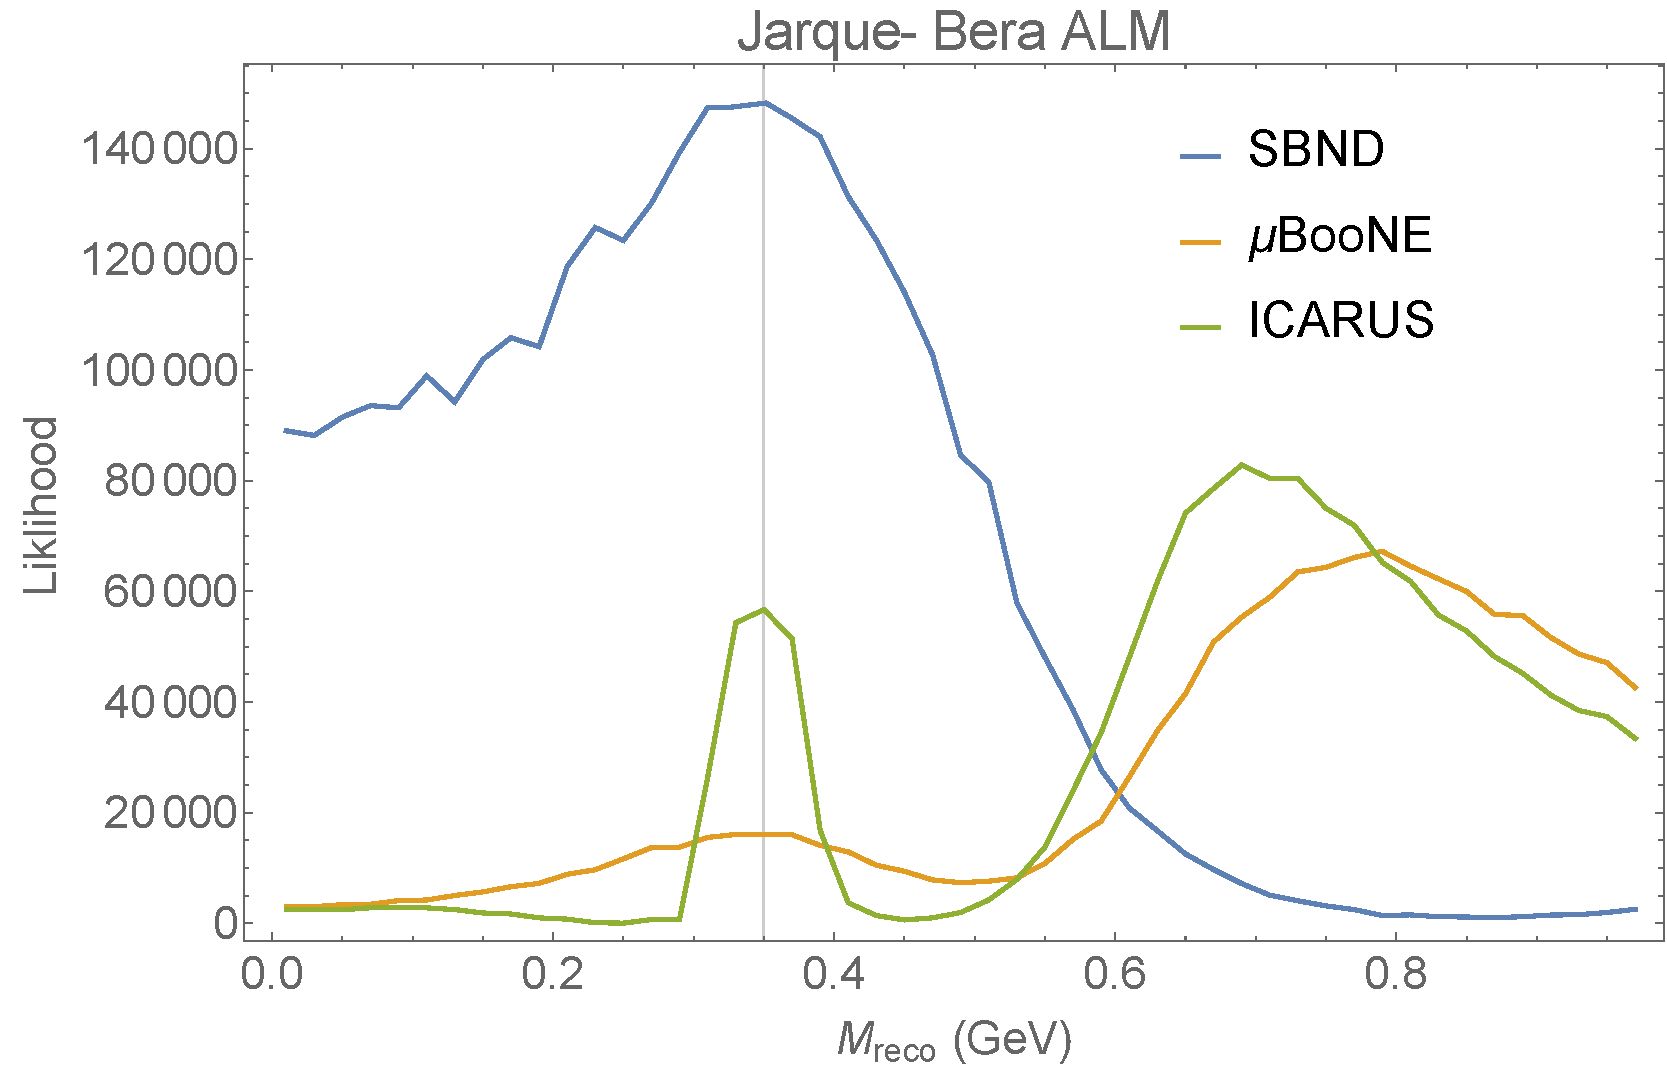
\includegraphics[width=0.7\textwidth]{figures/time_of_flight.pdf}
%\caption{\label{fig:tof} Ability of each of the SBN detectors to estimate the mass of a decaying particle, with $m_s^\text{true} = 0.350 $ GeV,  based on time of flight only. If $m_\text{hypothesis} \leq m_\text{true}$ one can always push the parent bucket further back in time to achieve a good fit, therefore discrimination power of the further detectors begins to fail. This begins to happen at large masses, $m_\text{hypothesis} \approx 0.6$ GeV, larger than those of interest in this study. Due to the bad timing resolution of $\mu$BooNE in comparason to ICARUS and SBND, it contributes little to this anaysis.}
%\end{figure}





\lorem\lorem

\section{Conclusions}

The Fermilab Short-Baseline Neutrino complex will further our knowledge of
neutrino beams at short-baseline and neutrino interactions. In this paper, we
have studied its capabilities to constrain decaying sterile neutrinos with
masses around the MeV scale. To make a fair assessment of the potential to
constrain these models, we have performed a cut-based analysis of the dominant
backgrounds and signals and shown that high levels of background suppression
can be expected, resulting in close to backgroundless searches. We have
identified the importance of timing on both the appearence of new signals and
the analysis of backgrounds to these signals. Using these background estimates,
we have performed a sensitivity analysis to the parameters of the minimal
extension of the SM with a novel sterile neutrino. We have also motivated
searches for non-minimal models, which in particular could lead to observable
decays over a wide range of parameter space which is conventionally excluded by
theoretical assumptions on the decay rates themselves. We argue that these
decay rates are actually \emph{unconstrained} in published work, and show that
the SBN could place the first bounds on these processes. We have then discussed
the role of the unique design of the SBN complex: the three detectors allow for
complicated interplay of effects, including scaling of event rates with
baseline or mass, and timing effects which allow for a thorough investigation
of an excess were it to be discovered. 


\acknowledgments

We would like to thank Andrezj Szelc for his input to various elements of this
work, and also to Jonathan Asaadi for helpful discussions at the start of this
project.

This work has been supported by the European Research Council under ERC Grant
“NuMass” (FP7-IDEAS-ERC ERC-CG 617143) and by the European Union FP7
ITN-INVISIBLES (Marie Curie Actions, PITN-GA-2011-289442).

\appendix

\section{To do list}

\begin{enumerate}

	\item \newtext{MARK}{Working on} Nice plots for signal kinematics. What do we want to show in the signal
section? Forwardness? Energy? 

\item Decide what statistical method to use? Do we do a spectral fit?

\item How does eventrate actually deal with spectra things? Can we modify it to 
do spectral plots or even fits?


\item \newtext{MARK}{Working on} Generagte efficiency file from above cuts.

\item \newtext{MARK}{Working on} Use the efficiency files from previous point to produce new plots of
sensitivity.

\item Implement $\nu\gamma$ decay rate. 

\item Compute plots for enhanced decay rates to unobserved channels. Check that
the enhanced $\Gamma$ code works.

\item Do a bit more checking that the `unobserved' channels are indeed unobserved.

\item Baseline dependence + event timing = physics? (Decide what we can do with
event ratios + scaling, or timing analysis).  \emph{e.g.} see figure
\ref{fig:baseline_comp}.

\item Timing scatterplots to distingush sterile masses, currently two mathematica notebooks with scatterplot and nautilus plot calculations on DropBox (not gitable).

\item Turn on $U_{\tau 4}$,$U_{\mu 4}$ and $U_{e4}$ simultaneously. Think of
how we can push the analysis beyond the obvious by using flavour effects. Also
look at ratios of channels and ratios of events to see if we can get any
(broken) degeneracies that could actually be interesting \emph{i.e} SNO style
complementary measurements.

\item Keep refining text. Add introduction; write sterile decay section; structure 
the simulation details section; write conclusions etc.

\item \newtext{MARK}{Working on} Make nice version of branching ratio plot. Need to make prettier. \sout{Also, we probably need to cut it off at 
	$M_N\lesssim 500$ MeV, there are other decays allowed between 0.5 and 1 GeV (with $\eta$ and $\rho$)}.

\item \newtext{MARK}{Working on} Think if there's a nice plot showing the sterile effect on our fluxes.

%\item Actually compute a $95\%$ CL exclusion region for a fair comparison with
%bounds. \newtext{PB}{See comment directly below. (This isn't a total
%solution... but I spent a while reading about how to do this properly and I
%think it's pretty defensible. Perhaps more so than what we would do with
%log-likelihood ratios...)}.
%
%\item \sout{The $S/\sqrt{B} =1$ criterion is (if it's defensible at all) really a
%$1\sigma$ significance measure. I think we should at least switch it to
%$S/\sqrt{B} =2$ which is $2\sigma\approx 95\%$ in the Gaussian limit.}
%\newtext{PB}{I have done this and updated the plotting scripts.}


	\end{enumerate}

%\begin{figure}[t]
%\center
%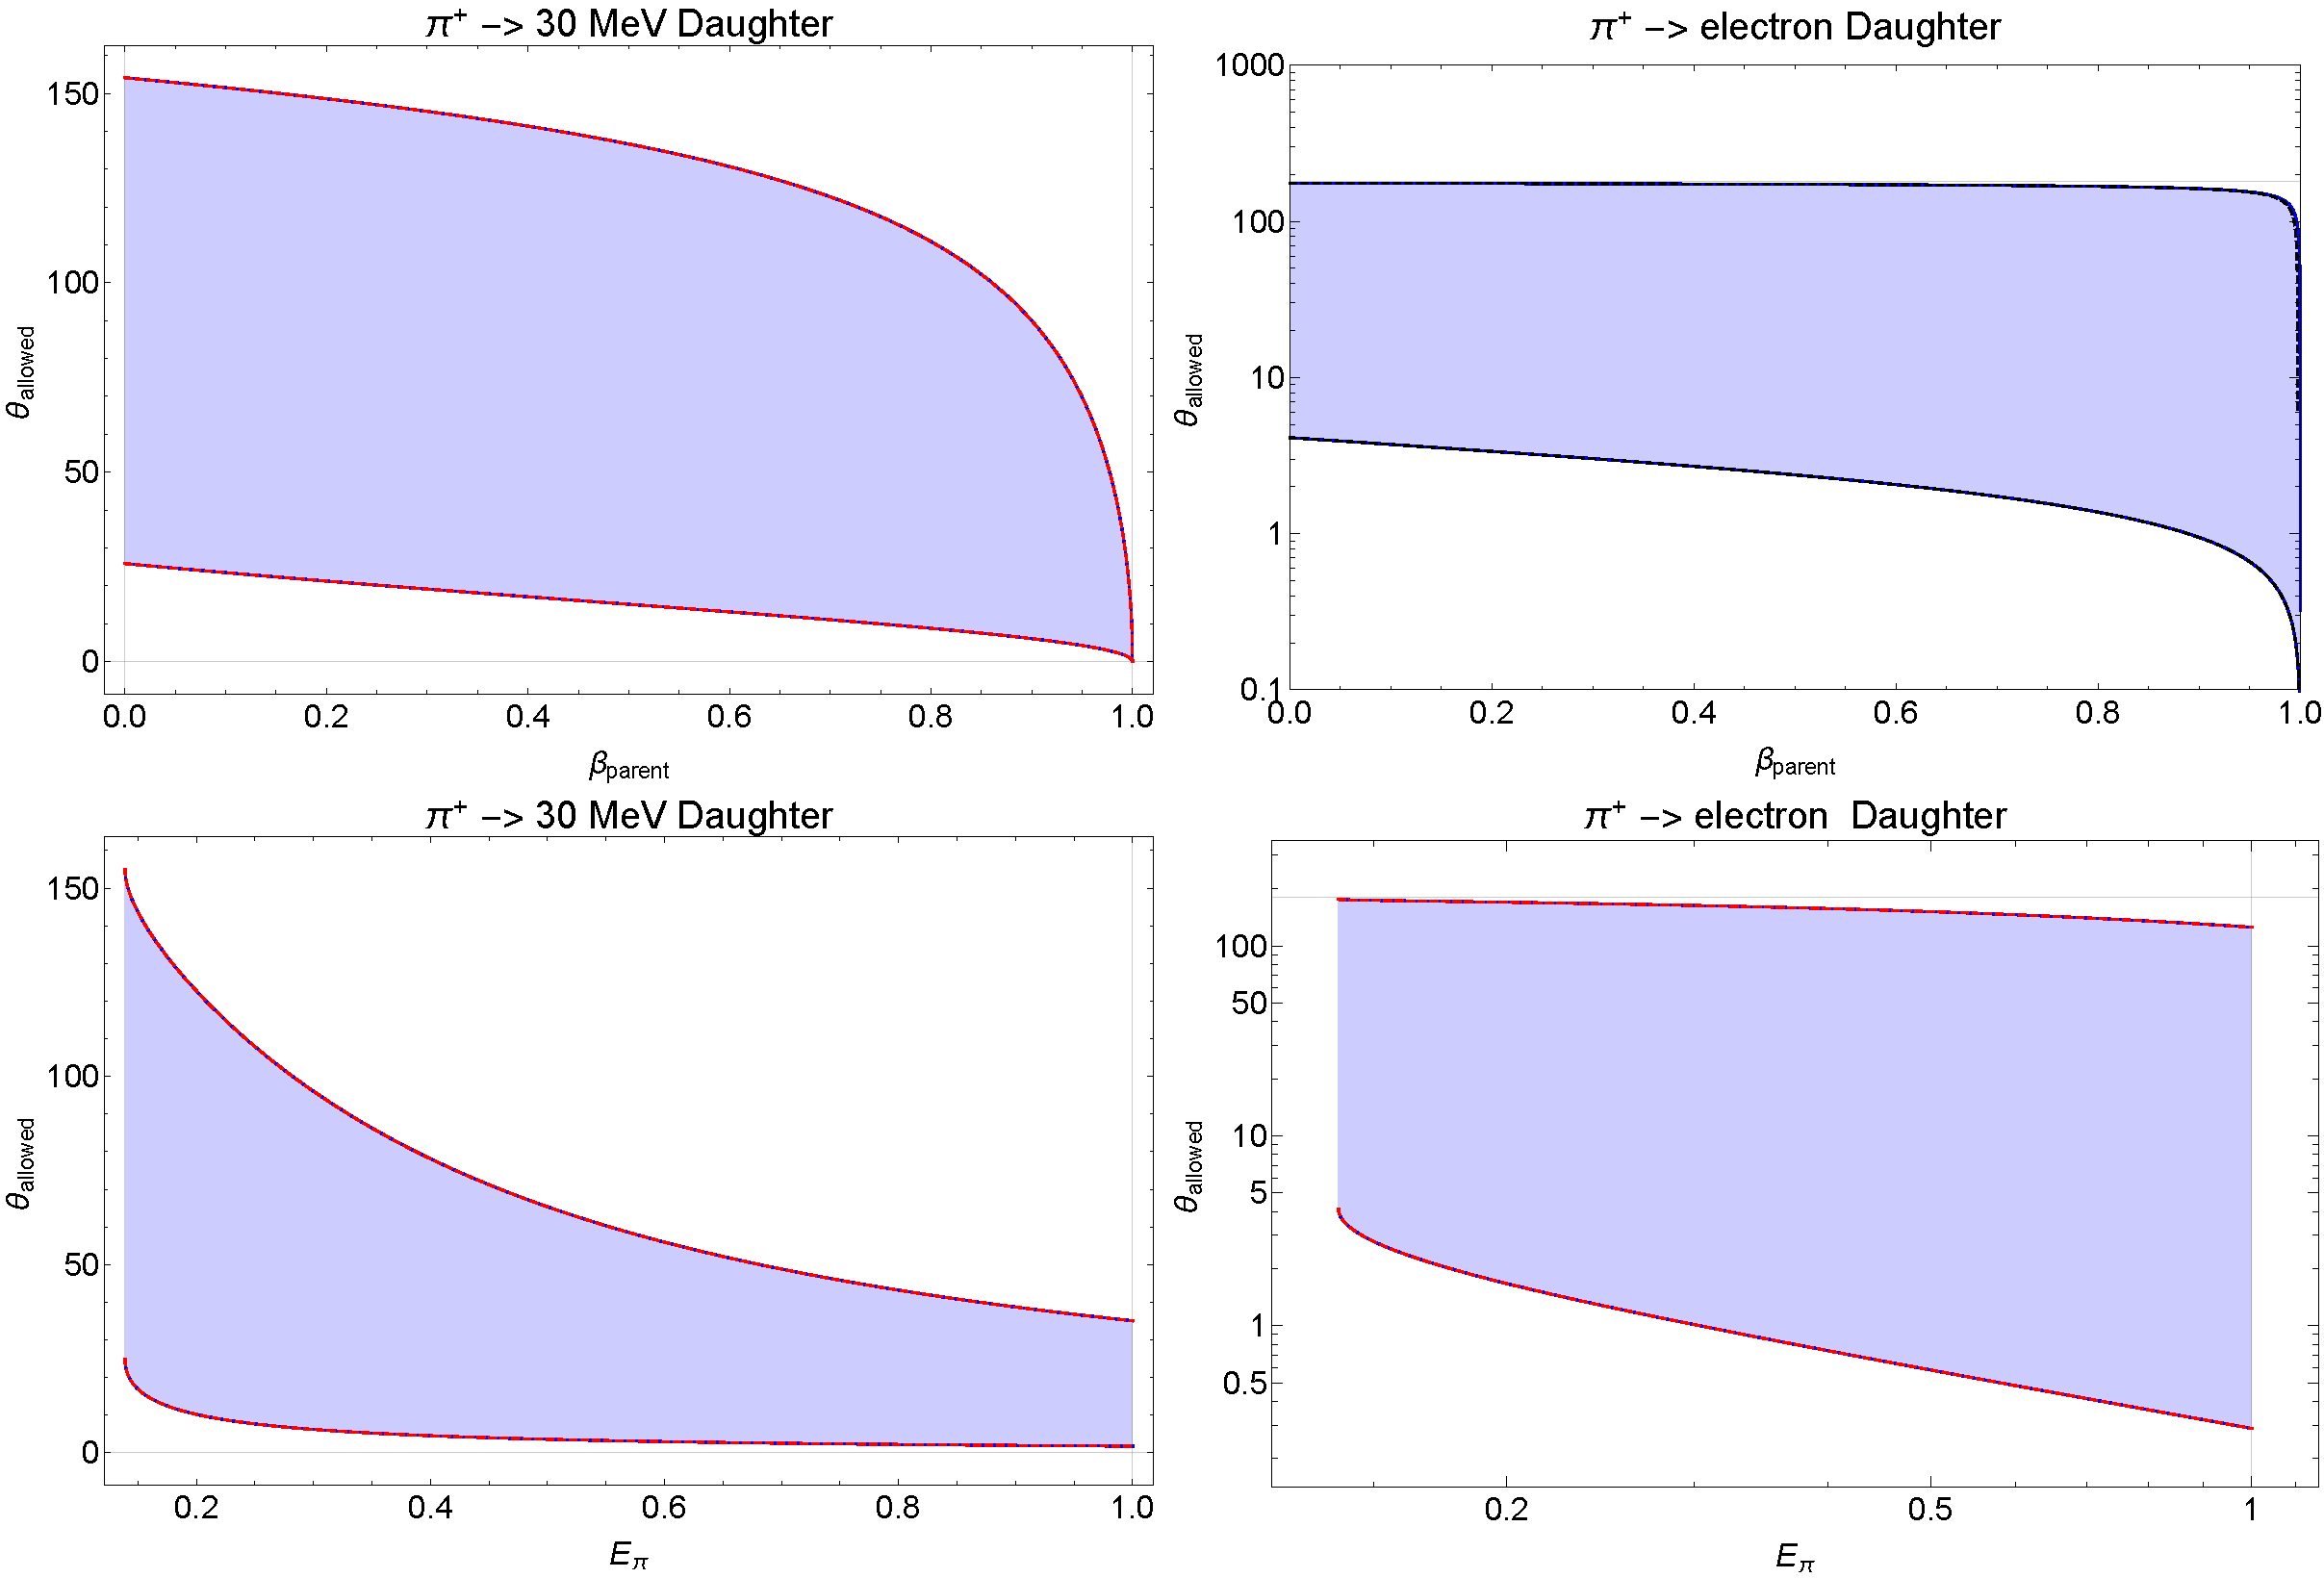
\includegraphics[width=1.0\textwidth]{figures/angles_boost.pdf}
%\caption{\label{fig:boost} Allowed angles in the decay $m_\pi \rightarrow a+b$ for $m_a 30$ MeV and $m_a=m_e$. In the limit of $m_a \rightarrow 0$ the entire $\beta_\pi - \theta_a$ plane is covered, which is pretty much what we were calculating today!   .}
%\end{figure}


	
%\begin{figure}[t]
%\center
%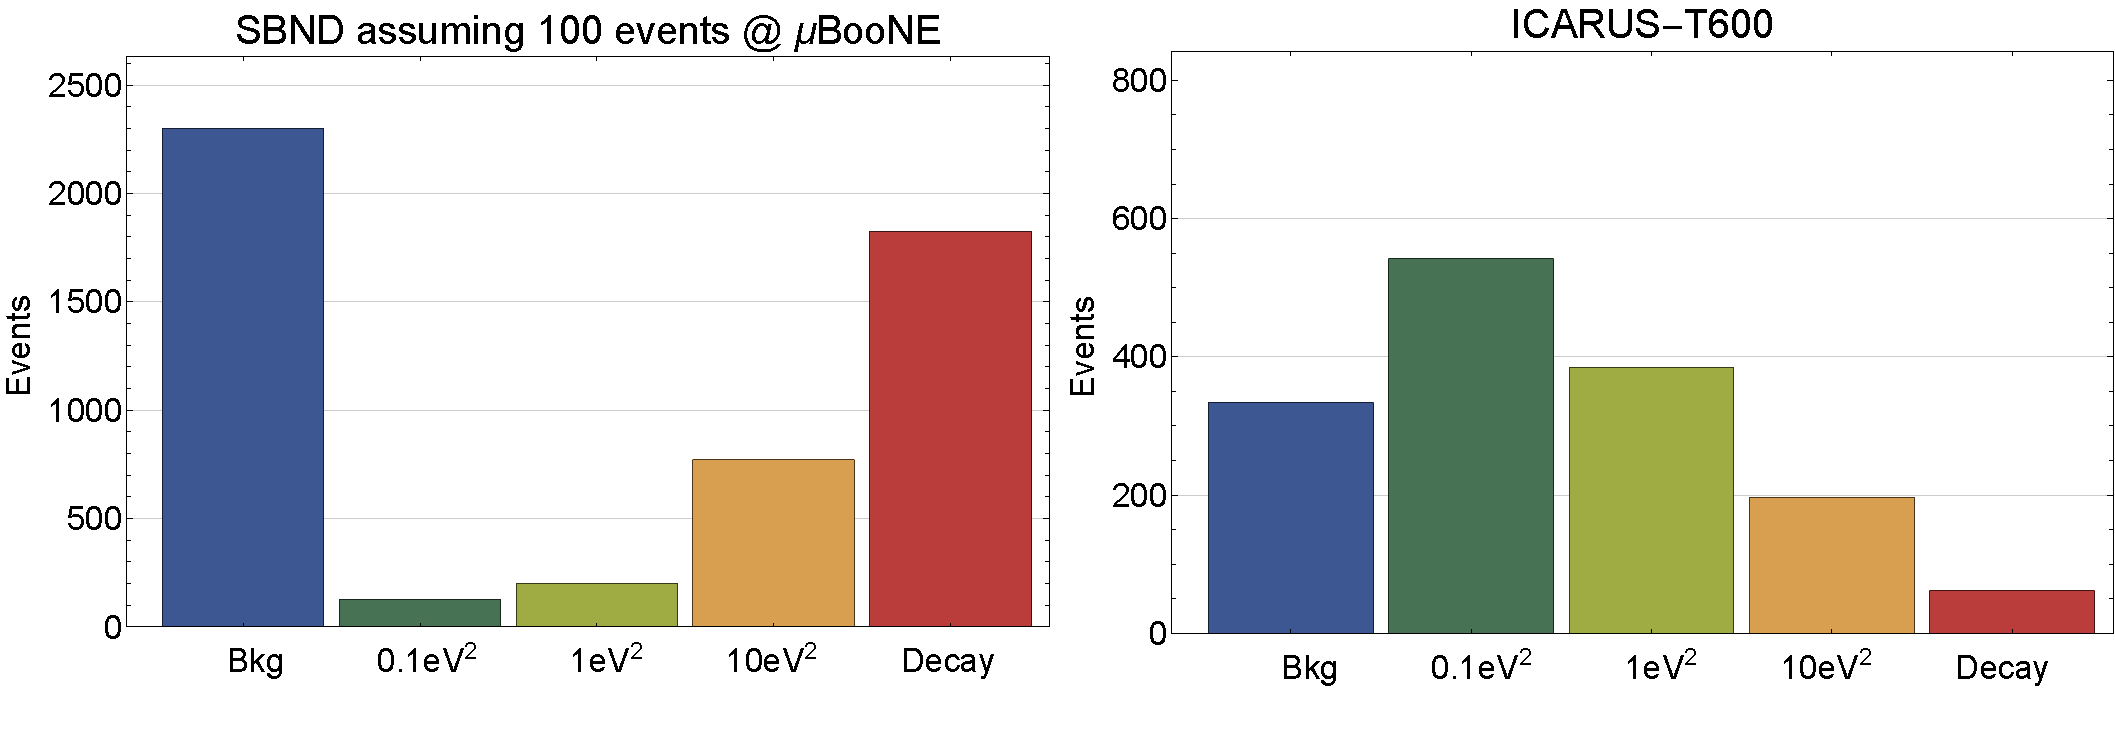
\includegraphics[width=0.7\textwidth]{figures/baseline_comp.pdf}
%\caption{\label{fig:baseline_comp} Assuming \muboone\ sees 100 events excess, what would SBND and Icarus see if the 100 events was truely a background event, an oscillating sterile of 0.1 $\text{eV}^2$, 1  $\text{eV}^2$ or 10 $\text{eV}^2$ or a decaying 100 MeV sterile n flight. }
%\end{figure}


%%%%%%%%%%%%%%%%%%%%%%%%%%%%%%%%
%%%%%%%%%%%%%%%%%%%%%%%%%%%%%%%%
%%%%%%%%%%%%%%%%%%%%%%%%%%%%%%%%

\bibliographystyle{apsrev4-1}
\bibliography{lib}{}

\end{document}

